% FYP Report
% article vs IEEEtran

% Packages
\documentclass[a4paper]{IEEEtran}
\usepackage{graphicx}
\usepackage{caption}	
\usepackage{enumerate}
\usepackage{hyperref}
\usepackage{mathpazo}
\usepackage{amsmath}
\usepackage{siunitx}
\usepackage{xspace}
\usepackage{subcaption}
\usepackage{algorithm,algorithmic}
\usepackage[skip=2pt,font=small]{caption}

% Math symbols
\let\Gamma\varGamma
\let\Delta\varDelta
\let\Theta\varTheta
\let\Lambda\varLambda
\let\Xi\varXi
\let\Pi\varPi
\let\Sigma\varSigma
\let\Upsilon\varUpsilon
\let\Phi\varPhi
\let\Psi\varPsi
\let\Omega\varOmega

% Commands
\newcommand{\RSonar}{$\si{\textit{R}_{s}}$\xspace} 
\newcommand{\ThetaSonar}{$\si{\Theta_{s}}$\xspace} 
\newcommand{\PhiSonar}{$\si{\Phi_{s}}$\xspace} 
\newcommand{\UCamera}{$\si{\textit{U}_{c}}$\xspace} 
\newcommand{\VCamera}{$\si{\textit{V}_{c}}$\xspace}
\newcommand{\XSonar}{$\si{\textit{X}_{s}}$\xspace}
\newcommand{\YSonar}{$\si{\textit{Y}_{s}}$\xspace}
\newcommand{\ZSonar}{$\si{\textit{Z}_{s}}$\xspace}
\newcommand{\Depth}{$D_{D}$\xspace}
\newcommand{\YDepth}{$Y_{D}$\xspace}

\newcommand{\RSonarVelocity}{$\dot{R}$\xspace} 
\newcommand{\ThetaSonarVelocity}{$\dot{\Theta}_{s}$\xspace} 
\newcommand{\PhiSonarVelocity}{$\dot{\Phi}_{s}$\xspace} 
\newcommand{\XSonarVelocity}{$\si{\dot{\textit{X}}_{s}}$\xspace}
\newcommand{\YSonarVelocity}{$\si{\dot{\textit{Y}}_{s}}$\xspace}
\newcommand{\ZSonarVelocity}{$\si{\dot{\textit{Z}}_{s}}$\xspace}

\newcommand{\XVehicle}{$\si{\textit{X}_{v}}$\xspace}
\newcommand{\YVehicle}{$\si{\textit{Y}_{v}}$\xspace}
\newcommand{\ZVehicle}{$\si{\textit{Z}_{v}}$\xspace}
\newcommand{\RollVehicle}{${\alpha_{v}}$\xspace}
\newcommand{\PitchVehicle}{${\beta_{v}}$\xspace}
\newcommand{\YawVehicle}{${\gamma_{v}}$\xspace} 
\newcommand{\RollVehicleVelocity}{${\dot{\alpha_{v}}}$\xspace}
\newcommand{\PitchVehicleVelocity}{${\dot{\beta_{v}}}$\xspace}
\newcommand{\YawVehicleVelocity}{${\dot{\gamma_{v}}}$\xspace} 
\newcommand{\XVehicleVelocity}{$\si{\dot{\textit{X}}_{v}}$\xspace}
\newcommand{\YVehicleVelocity}{$\si{\dot{\textit{Y}}_{v}}$\xspace}
\newcommand{\ZVehicleVelocity}{$\si{\dot{\textit{Z}}_{v}}$\xspace}

% Settings
%\setlength{\parindent}{1em}
%\setlength{\parskip}{0.2em}
%\setlength{\belowcaptionskip}{-20pt}
%\setlength{\textfloatsep}{10pt plus 1.0pt minus 2.0pt}
\newcolumntype{C}[1]{>{\centering\arraybackslash$}m{#1}<{$}}
\newlength{\mycolwd}                                         % array column width
\settowidth{\mycolwd}{$e^{-\frac{i}{\hbar}|A|t}$}% "width" of $e^{-\frac{i}{\hbar}|A|t$; largest element in array
\settowidth{\mycolwd}{$e^{-\frac{i}{\hbar}|A|t}$}
\newcommand\w[1]{\makebox[\mycolwd]{$#1$}}
\newcommand\scalemath[2]{\scalebox{#1}{\mbox{\ensuremath{\displaystyle #2}}}}
\arraycolsep=3pt % default: 5pt
\medmuskip = 1mu % default: 4mu plus 2mu minus 4mu

% Title and Authors
\title{
Underwater Target Tracking using Forward Looking Sonar (FLS) and Optical Camera via Calibration and Particle Filter Fusion
}
\author{
National University of Singapore \\
Yaadhav Raaj, Dr. Ng Tek Khim
}

% Document Begins
\begin{document}
\maketitle

% Font size
\small

% Abstract
\begin{abstract}
Underwater Target tracking is widely used in the industry in Autonomous Underwater Vehicles (AUV), both in sea and lake environments for various applications. Sonars and Cameras are popular choices for this, but each sensor alone poses several problems. Optical Cameras are challenging due to poor lighting conditions, hazing over large distances and spatio-temporal irradiate (flickering), while Sonars tend to have coarser sensor resolution and a lower signal-to-noise ratio (SNR) making it difficult to extract data. These makes false positives more likely. Also, it's not possible to perceive the 3D coordinates of objects from either one alone. In this paper, we present a robust method to track and detect stationary objects from the camera imagery, sonar imagery and odometry information from onboard sensors in 3D space. This is done through various image processing techniques, a pre-calibration step, and finally a particle filter based approach for data fusion.
\end{abstract}

\section{Introduction}
Vision plays a key role in object localization in underwater environments. Object localization in such environments is used extensively in AUV's, for commercial applications such as undersea pipeline analysis for the oil and gas industry, or scientific research such as the study of marine life. Many of these applications require the vehicle to move towards a target and get close enough before performing more complex tasks. In order to perform this localization step, having AUV's equipped with sonars and optical cameras have become a standard practice. 

Optical cameras are extensively used for this purpose, where one can make use of various image processing algorithms to find a region of interest (ROI) and it's centroid (\UCamera, \VCamera) to track. However, finding this from the image alone is difficult. In shallow environments, noise can be attributed to spatio-temporal irradiance (flickering) and scattering [1]. This makes algorithms for thresholding or segmentation work ineffectively, which makes tracking difficult. In deep environments, hazing due to low light conditions and suspended particles in the water make segmentation via Edge based or HSV color space based segmentation difficult [2]. Bianco [2] uses the dark channel prior estimate to dehaze the scene, and get a depth map as well, but this method cannot run in real time. Camera's are unable to perceive depth or bearing without resorting to Structure from Motion (SFM) or Stereo Camera techniques, both which require good features to track and hence are are susceptible to the issues above.

Sonars are also extensively used for this purpose. Two popular models in ROV's/AUV's are the DIDSON (Dual-Frequency Identification Sonar) and the Teledyne Blueview series, based on blazed array technology. The sonar used here is the Blueview P450-E [3]. It is able to provide video imagery at up to 12Hz, and has a maximum Range (\RSonar), Azimuth (\ThetaSonar), and Elevation (\PhiSonar) of 200m, 45\si{\degree} and 15\si{\degree} respectively.  Similar algorithms are used to extract Range (\RSonar) and Azimuth (\ThetaSonar) of objects from the sonar imagery.  However, the coarser sensor resolution combined with the lower signal-to-noise ratio (SNR) make data extraction challenging. Reflections from walls, or waves on the water surface produce large amount of noise. Furthermore, most mid-range systems such as the one used here are unable to provide Elevation (\PhiSonar) data, making it impossible to compute 3D coordinates, and hence correct for depth.

The visibility limitations, intermittent loss of data due to high SNR and lack of 3D information of the object make localizing and tracking these objects difficult. In this paper, we propose a novel method for fusing information from the camera and sonar imagery, along with odometry information from the vehicle using particle filters to track and detect objects, assuming prior information such as the dimensions and color of said object is provided.

\begin{figure}[h!]
  \centering
  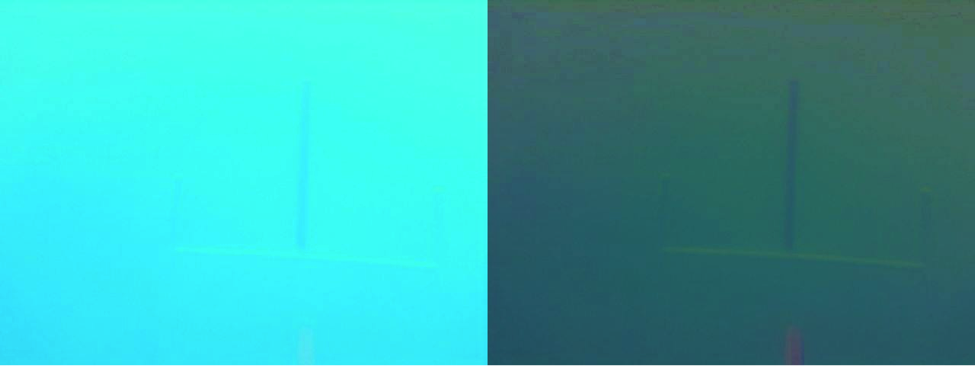
\includegraphics[scale=0.5]{imageUnderwater}
  \captionsetup{justification=centering}
  \caption{Poor image quality even after dehazing and contrast enhancement techniqies}
\end{figure}

This paper assumes that both sensors are arranged with overlapping views, and hence it would be possible to model the transformational geometry between both spaces. It assumes that sonar is factory calibrated, and that a pre-calibration step on the camera is performed to find it's intrinsic matrix. The premise is to acquire (\RSonar, \ThetaSonar) and (\UCamera, \VCamera) from the sonar and camera data to compute the 3D coordinates (\XSonar, \YSonar, \ZSonar) in the sonar frame, which is then used for path planning purposes. Lastly, it assumes that odometry information, such as angles of rotation (\RollVehicle, \PitchVehicle, \YawVehicle), angular velocities (\RollVehicleVelocity, \PitchVehicleVelocity, \YawVehicleVelocity), translational velocities (\XVehicleVelocity, \YVehicleVelocity, \ZVehicleVelocity), and depth (\Depth) from the water surface are known, possibly through the use of a Doppler Velocity Log (DVL), Inertial Measurement Unit (IMU), and pressure sensor about the vehicle centre of mass (COM). These are assumed to be calibrated as well. 

\section{Preliminaries}

\subsection{Literature Review}
Many previous sensor fusion approaches that used range and bearing (LIDAR, RADAR, SONAR) with an optical camera have been tested and used well-defined environments with many features to track, where the sonar points towards the surface but not ahead [4][5]. In the seminal paper describing 3D mapping of the great barrier reef [4], the transformations between the sensors appear to be already known/calibrated, and the bottom camera feed has significant features to track in order to perceive range and is at close proximity to the objects of interest. This might not be the case in the forward range where objects are much further away. However, many useful ideas, such as projection of the sonar features into the camera frame, and involving of vehicular ego motion in tracking of the stationary objects are later used in this paper.

\begin{figure}[h!]
  \centering
  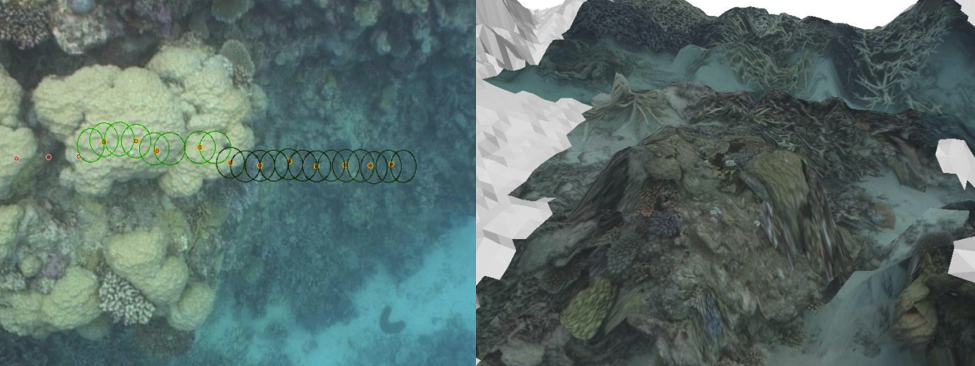
\includegraphics[scale=0.5]{reef}
  \captionsetup{justification=centering}
  \caption{3D map generation using sonar and camera on the Great Barrier Reef}
\end{figure}

Since the FLS does not provide elevation information, methods such as projecting the sonar ambiguity space has also been done. In Anthony Spear’s paper [6], where the use case was for tracking underwater ice systems in the artics, objects detected in the sonar data are mapped directly into the camera image as an area of interest in which to search for landmarks. Although a precise calibration method is not used here, both sensor's field of view is used to determine a bounding box where the object may exist in the camera frame. Such ideas were used in the paper as well. However, this method may not have been enough to localize precisely or acquire said objects 3D coordinates.

\begin{figure}[h!]
  \centering
  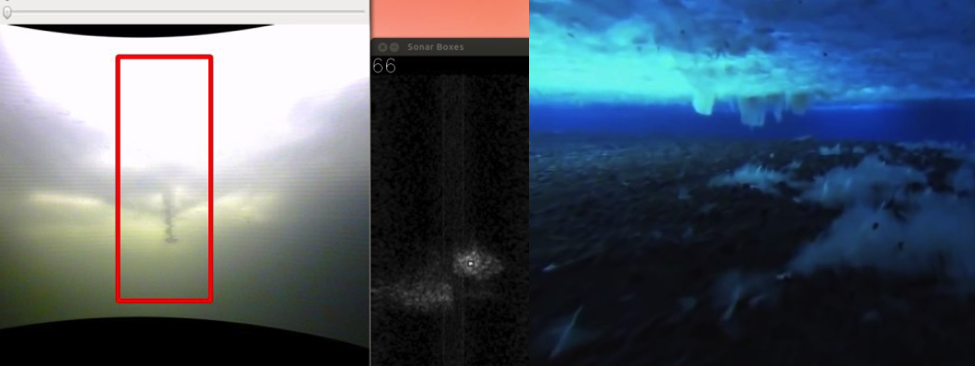
\includegraphics[scale=0.5]{ice}
  \captionsetup{justification=centering}
  \caption{Project sonar image into camera space on under ice topography}
\end{figure}

Motion tracking approaches fusing information from sonar and camera data using a Joint Probabilistic Data Association (JDPA) fusion approach has also been studied [7]. Information from the camera is used to correct the position of the floating buoy in a planar space. This method works well as the camera is on the surface, allowing better tracking on that space. However, our use case requires the system to track objects in 3D space while fully submerged, and fusion in 2D space may only aid in visual servoing which is not the intention.

\begin{figure}[h!]
  \centering
  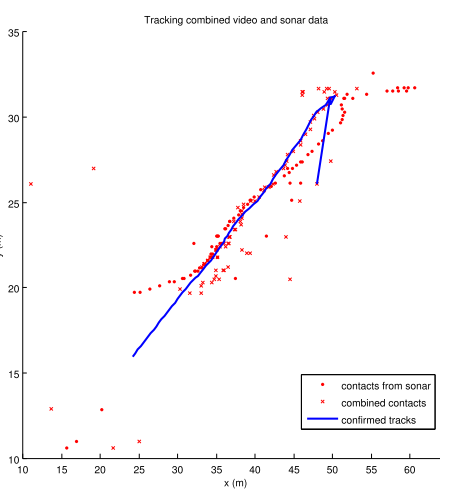
\includegraphics[scale=0.4]{jdpa}
  \captionsetup{justification=centering}
  \caption{The red dots are the contacts from the sonar, the red x’s are the contacts that result from fusing the sonar and video data, and the blue line is the confirmed track from the JPDA tracking algorithm}
\end{figure}

Lastly, state of the art calibration techniques between sonar and camera spaces by S. Negahdaripour have also been extensively studied [8] [9]. In these papers, opti-acoustic feature matching and the epipolar geometry between both sensors is discussed. The equations describing both sensor spaces include the polar to cartesian conversions of the sonar space, transformation matrix between both sensors, perspective projection of 3D points into the camera space as pixels and a closed formed solution solving for \PhiSonar. The paper describes the use of the Levenberg Marquardt algorithm [10] for non-linear optimization in order to solve for the unknown transformation parameters, and also shows the use of a special calibration grid. Although a much simplified model is used later on for our use case, many ideas are taken from these two papers.

\begin{figure}[h!]
  \centering
  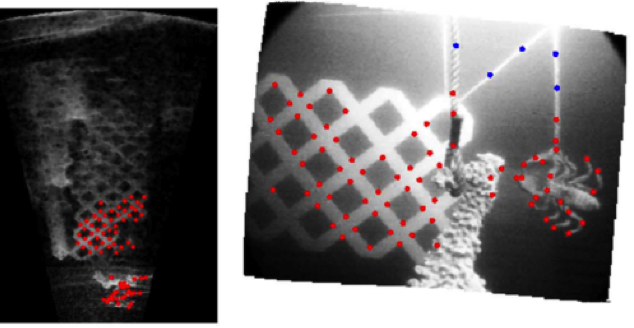
\includegraphics[scale=0.3]{sonarcam}
  \captionsetup{justification=centering}
  \caption{Corresponding points between sonar and camera images}
\end{figure}

\subsection{Vehicle}

\begin{figure}[h!]
  \centering
  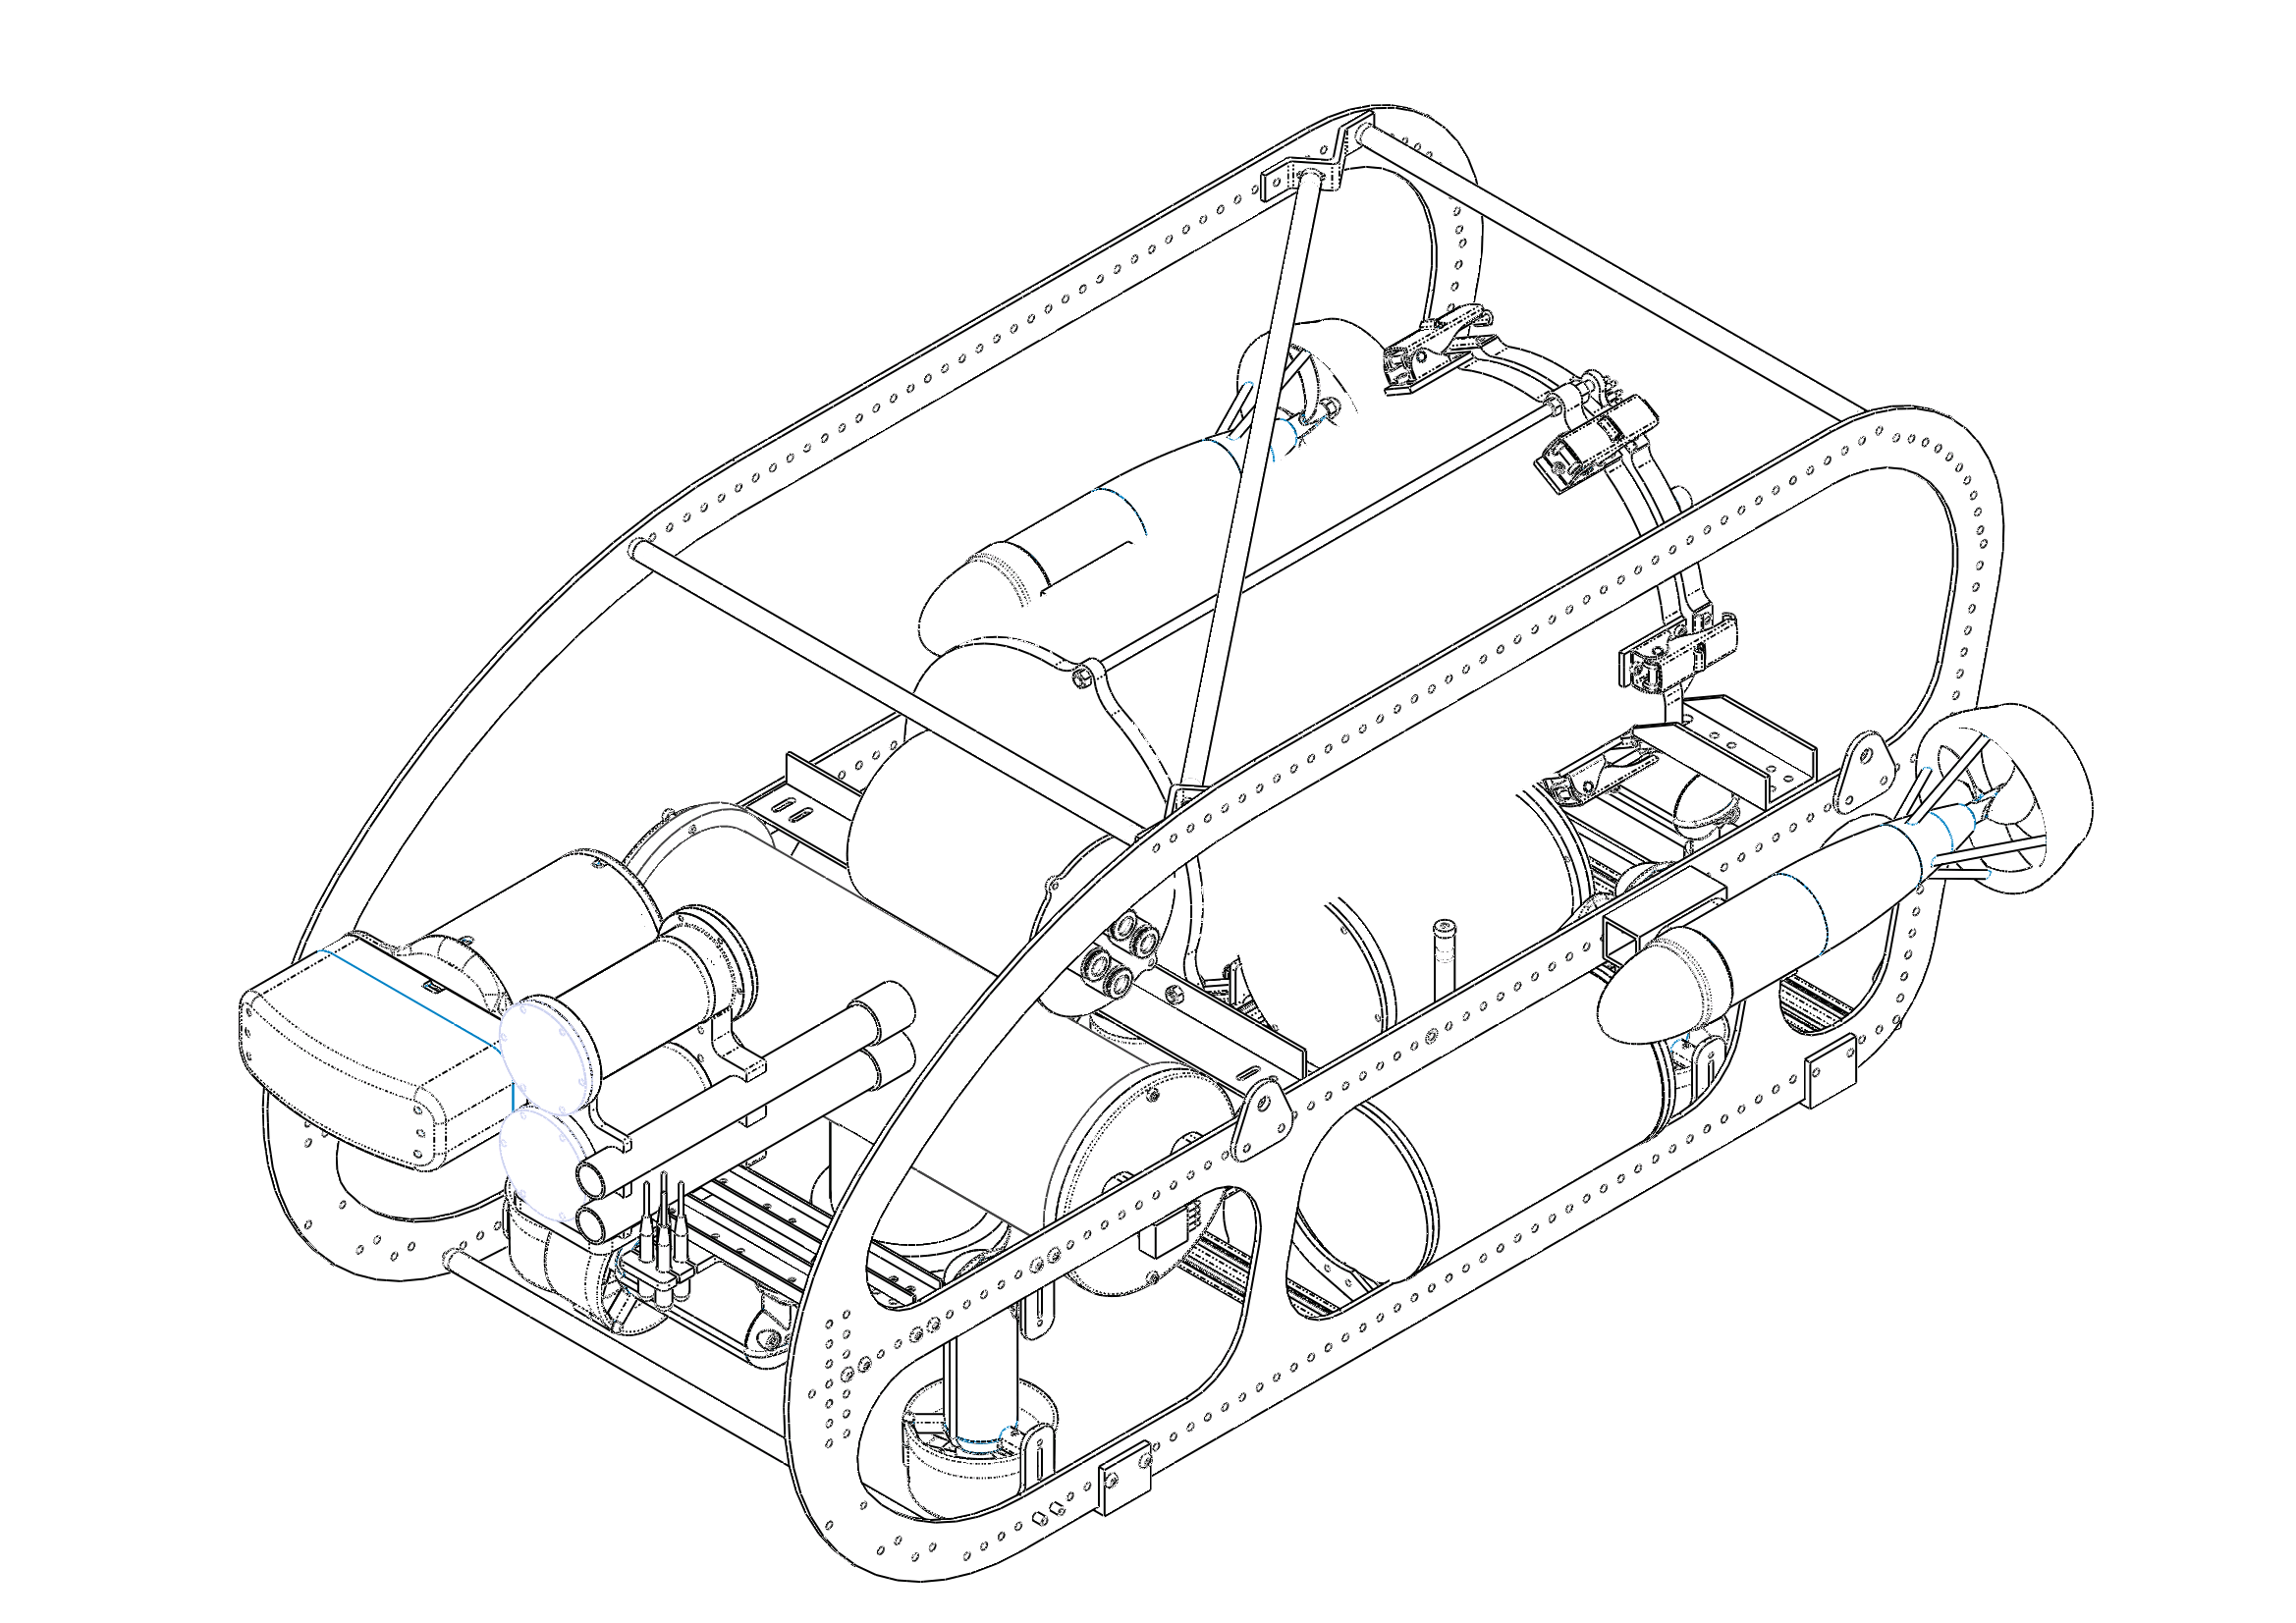
\includegraphics[scale=0.2]{bbauv25}
  \captionsetup{justification=centering}
  \caption{BumbleBee AUV 2.5}
\end{figure}

\begin{table}[h]
\resizebox{\columnwidth}{!}{%
\begin{tabular}{|l|l|}
\hline
{\bf Weight}                & 50 kg                                                                                                                \\ \hline
{\bf Dimensions}            & 0.7m X 1.1m X 0.5m                                                                                                   \\ \hline
{\bf Single Board Computer} & \begin{tabular}[c]{@{}l@{}}Core i7 - 3610QE\\ Aaeon EMB-QM77\\ 8GB DDR3 RAM\\ 512GB SATA3 SSD\end{tabular}           \\ \hline
{\bf Embedded System}       & \begin{tabular}[c]{@{}l@{}}Arduino Mega 2560\\ Xilinx Spartan-3 on NI sbRIO 9602\end{tabular}                        \\ \hline
{\bf Propulsion}            & \begin{tabular}[c]{@{}l@{}}6 SeaBotix BTD150\\ 2 VideoRay Surge Thrusters\end{tabular}                               \\ \hline
{\bf Navigation}            & \begin{tabular}[c]{@{}l@{}}Teledyne RDI Explorer DVL\\ Sparton GEDC-6 IMU\\ US300 Pressure/Depth Sensor\end{tabular} \\ \hline
{\bf Vision Sensors}        & \begin{tabular}[c]{@{}l@{}}AVT Guppy Pro\\ AVT Guppy\end{tabular}                                                    \\ \hline
{\bf Sonar}                 & \begin{tabular}[c]{@{}l@{}}BlueView P450 Imaging Sonar\\ 4 Teledyne Reson TC4013 Hydrophones\end{tabular}            \\ \hline
{\bf Manipulators}          & Festo Pneumatics Systems                                                                                             \\ \hline
{\bf Power Supply}          & 22.2V 10000mAh LiPo Battery (x2)                                                                                      \\ \hline
{\bf Underwater Connectors} & SubConn Micro and Low Profile Series                                                                                 \\ \hline
{\bf Software Architecture} & \begin{tabular}[c]{@{}l@{}}Robot Operating System (ROS)\\ Debian GNU/Linux x64\end{tabular}                          \\ \hline
\end{tabular}
} \\
\caption{BumbleBee AUV 2.5 Specifications}
\end{table}

The vehicle used for testing is the Bumblebee Autonomous Underwater Vehicle (BBAUV) [11]. BBAUV is equipped with a Guppy Pro F-503 5 Megapixel Color CMOS Camera, Blueview P450-E Imaging Sonar for vision, Teledyne TDI Explorer DVL (Doppler Velocity Log), Sparton AHRS-8 IMU, Reson TC4013 hydrophones and a depth sensor for navigation and acoustics, and 2 VideoRay and 6 SeaBotix Thrusters for up to 6DOF. Fusion of the DVL and IMU via an Extended Kalman Filter provides odometry information and allows the vehicle to move to any 3D Coordinate. The US300 pressure depth sensor provides depth with an accuracy of +-1cm. The sonar, camera and odometry sensors lie in the same rigid body frame where the transformations between them is known through the mechanical model. This information will be later used as initial values for the calibration process.

\subsection{Sonar Model}

\begin{figure}[h!]
  \centering
  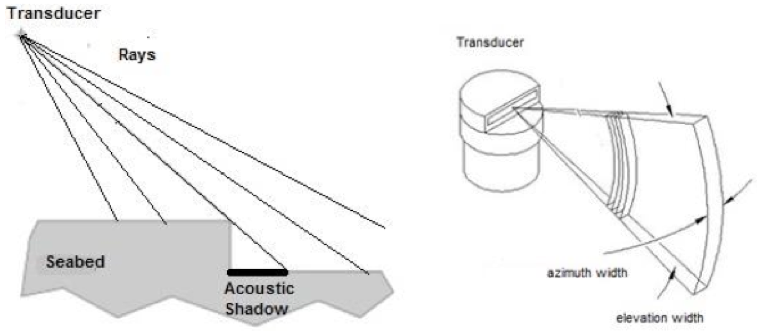
\includegraphics[scale=0.2]{sonar3}
  \captionsetup{justification=centering}
  \caption{FLS Image Formation}
\end{figure}

Concepts and equations behind the FLS are based off the “Springer handbook of robotics” [12] while understanding of formation of FLS imagery is based off [13]. An FLS is made of an array of vertical and horizontal transducers, which generate pulses of high frequency noise (450 Khz for the P450-E). The FLS Model is usually represented in spherical coordinates of azimuth, elevation angles, and range. They are also equipped with multiple transducers (The P450-E has 256 transducers). Each individual transducer can be represented as an optical ray, where the azimuth and elevation are 1\si{\degree} and 15\si{\degree} respectively as seen from Fig. 7. Hence, the horizontal beam spacing is about 256/45=0.18\si{\degree}. 

Sonar’s form images using time of flight of pulses. Each transducer output/ray can be plotted as a function of time which consists of both Intensity and Range as seen from Fig. 8. Objects that are further away have a lower intensity due to signal attenuation in the medium. Also, there is a possibility that two objects at different \PhiSonar but same \RSonar may overlap in the image causing it to be impossible to perceive both objects separately. Furthermore, reflections from walls may result in objects appearing further than they actually are.

\begin{figure}[h!]
  \centering
  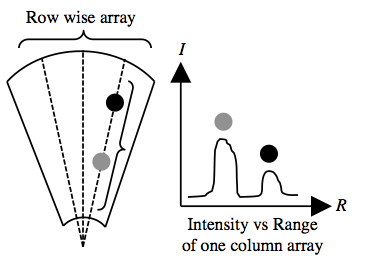
\includegraphics[scale=0.4]{transducers}
  \captionsetup{justification=centering}
  \caption{FLS Image Formation}
\end{figure}

Intensity of the object is also dependant on the angular deviation from the line-of-sight of the transducer [14].  $\lambda$ is the sound wavelength, a and b are respectively the length and the width of the aperture of the transducer, $\alpha$ and $\beta$ are the coordinates of the vector of angular deviation (Fig. 1), and Io(R) is the sound intensity at range R on the beam axis as seen from Eq. 1. Assuming the vehicle has an operating depth of less than 100m, based on the depth profile, it would have a $\lambda$ of 450khz/1500 = 0.003m.
\begingroup\makeatletter\def\f@size{7}\check@mathfonts
\begin{gather}
I\left( R,\theta  \right)\; =\; I_{0}\left( R \right)\left( \frac{\sin \; p}{p} \right)^{2}\left( \frac{\sin \; q}{q} \right)^{2} \\
p\; =\; \frac{\pi a\alpha }{\lambda }\; q\; =\; \frac{\pi b\beta }{\lambda }\; 
\end{gather}
\endgroup
 
Lastly, the geometry of the object can be represented by Fig. 9 and Eq. 3. Here, we represent the sonar frame and the object coordinates in that frame in both cartesian and polar form. An alternative form is also used in this case, as the sensor inputs to form the 3d position of the object happen to be \RSonar, \ThetaSonar and \YSonar. \PhiSonar is not a sensor output provided by the sonar and is actually a value we wish to solve for later in the paper.
\begingroup\makeatletter\def\f@size{7}\check@mathfonts
\begin{gather}
\left[ \begin{array}{c} X_{s} \\ Y_{s} \\ Z_{s} \end{array} \right]\; =\; \left[ \begin{array}{c} R_{s}\cdot \cos \left( \phi _{s} \right)\cdot \sin \left( \theta _{s\; } \right) \\ R_{s}\cdot \sin \left( \phi _{s} \right) \\ R_{s}\cdot \cos \left( \phi _{s} \right)\cdot \cos \left( \theta _{s\; } \right) \end{array} \right]\; =\; \left[ \begin{array}{c} \sqrt{R_{s}^{2}\; -\; Y_{s}^{2}}\cdot \sin \left( \theta _{s\; } \right) \\ Y_{s} \\ \sqrt{R_{s}^{2}\; -\; Y_{s}^{2}}\cdot \cos \left( \theta _{s\; } \right) \end{array} \right]\; 
\end{gather}
\endgroup

\begin{figure}[h!]
  \centering
  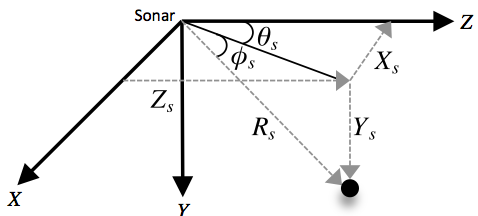
\includegraphics[scale=0.4]{sonarframe}
  \captionsetup{justification=centering}
  \caption{Sonar Frame}
\end{figure}

\subsection{Camera Model}

\begin{figure}[h!]
  \centering
  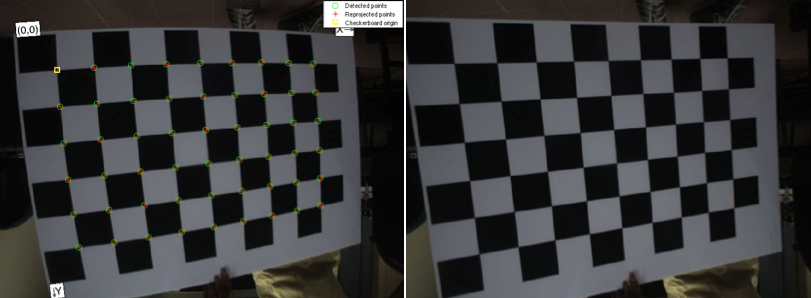
\includegraphics[scale=0.3]{camera}
  \captionsetup{justification=centering}
  \caption{Camera Calibration}
\end{figure}

The camera is geometrically calibrated via Zhang’s method [15] using a checkerboard pattern. Multiple checkboards are images are used, and are used to estimate the camera’s distortion parameters and instrinsic matrix. This allows us to map real world coordinates onto the camera plane by finding the focal lengths and principal points as seen in Eq. 4. To account for camera distortion, the radial coefficients (K Values) are also estimated using Brown-Conrady model as seen in Eq. 6. The results and the equations used are are shown below:
\begingroup\makeatletter\def\f@size{7}\check@mathfonts
\begin{gather}
\left[\begin{array}{c}
U_{c}\\
V_{c}
\end{array}\right]=\left[\begin{array}{cccc}
f_{x} & 0 & c_{x} & 0\\
0 & f_{y} & c_{y} & 0\\
0 & 0 & 1 & 0
\end{array}\right]*\left[\begin{array}{c}
X_{c}\\
Y_{c}\\
Z_{c}\\
1
\end{array}\right]=>\left[\begin{array}{c}
\frac{(f_{x}*X_{c})+(c_{x}+Z_{c})}{Z_{c}}\\
\frac{(f_{y}*Y_{c})+(c_{y}+Z_{c})}{Z_{c}}
\end{array}\right] \\
r=\sqrt{((U_{D}-c_{x})/f_{x})^{2}+((V_{D}-c_{y})/f_{y})^{2}} \\
\left[\begin{array}{c}
U_{U}\\
V_{U}
\end{array}\right]=\left[\begin{array}{c}
f_{x}*(((U_{D}-c_{x})/f_{x})*(1+K_{1}*r^{2}+K_{2}*r^{4}))+c_{x}\\
f_{y}*(((V_{D}-c_{y})/f_{y})*(1+K_{1}*r^{2}+K_{2}*r^{4}))+c_{y}
\end{array}\right]
\end{gather}
\endgroup  

\subsection{Combined Model}

\begin{figure}[h!]
  \centering
  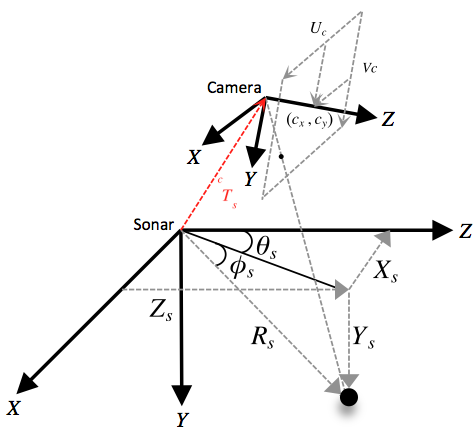
\includegraphics[scale=0.4]{sonarcamframe}
  \captionsetup{justification=centering}
  \caption{Sonar Camera Model}
\end{figure}

Now that we have an equation that can map 3D coordinates in the camera frame to camera pixels, we are able to combine both spaces based on Figure 11. This assumes that we know $^{c}T_{s}$ which may be roughly estimated from physical measurements. 
\begingroup\makeatletter\def\f@size{7}\check@mathfonts
\begin{gather}
\left[\begin{array}{c}
U_{c}\\
V_{c}
\end{array}\right]<=\left[\begin{array}{cccc}
f_{x} & 0 & c_{x} & 0\\
0 & f_{y} & c_{y} & 0\\
0 & 0 & 1 & 0
\end{array}\right]* \nonumber\\
\left[\begin{array}{cccc}
^{c}T_{s11} & ^{c}T_{s12} & ^{c}T_{s13} & ^{c}T_{s14}\\
^{c}T_{s21} & ^{c}T_{s22} & ^{c}T_{s23} & ^{c}T_{s24}\\
^{c}T_{s31} & ^{c}T_{s32} & ^{c}T_{s33} & ^{c}T_{s34}\\
0 & 0 & 0 & 1
\end{array}\right]
*\left[\begin{array}{c}
\sqrt{R_{s}^{2}-Y_{s}^{2}}\cdot\sin\left(\theta_{s}\right)\\
Y_{s}\\
\sqrt{R_{s}^{2}-Y_{s}^{2}}\cdot\cos\left(\theta_{s}\right)\\
1
\end{array}\right]
\end{gather}
\endgroup

\begin{figure}[h!]
  \centering
  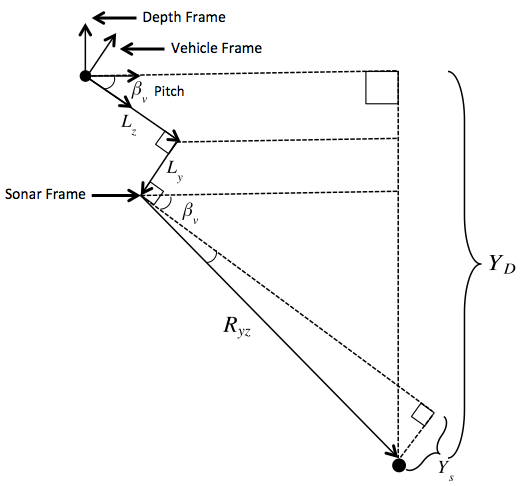
\includegraphics[scale=0.4]{sonarvehframe}
  \captionsetup{justification=centering}
  \caption{Sonar Vehicle Model}
\end{figure}

The depth sensor is located about the vehicle centre of mass (COM). Assuming the depth of the object of interest is measured, and the depth of the vehicle (\Depth) is known, we can easily derive the depth of the object relative to the vehicle COM aligned to the water surface (\YDepth). The depth sensor's output is assumed to be impervious to vehicular dynamics as it is placed at the vehicle COM, and it's frame is assumed to be aligned to the water surface. Using geometrical methods, we derived an equation that approximately maps \YDepth to \YSonar and vice-versa based on Fig. 12 and Eq. 9,10 using \RSonar and \PitchVehicle. $L_{z}$ and $L_{y}$ can also be estimated from physical measurements. ($R_{yz}$) is the flattened range of the $Y_{s}$ and $Z_{s}$ axis on the sonar frame and is approximately equal to $(R_{s}*\Theta_{s})$. Based on a workspace of a max $R$ of 15m and the sonar parameters listed in Eq. 8, we get a maximum error of 1.35cm and is deemed acceptable. Also, this model assumes that the roll effect is minimal which was the case in our vehicle.
\begingroup\makeatletter\def\f@size{7}\check@mathfonts
\begin{gather}
\left[\begin{array}{c}
\max\left(R_{s}\right)=15\\
\max\left(\theta_{s}\right)=45/2\\
\max\left(\phi_{s}\right)=15/2
\end{array}\right]\quad R_{yz}=R_{s}*cos(\Theta_{s})\\
Y_{D}=L_{y}*\cos\left(\beta_{v}\right)+L_{z}*\sin\left(\beta_{v}\right)+R_{yz}*\sin\left(\beta_{v}+\mbox{asin}\left(\frac{Y_{s}}{R_{yz}}\right)\right) \\
Y_{s}=-R_{yz}*\sin\left(\beta_{v}+\mbox{asin}\left(\frac{\left(L_{y}*\cos\left(\beta_{v}\right)-Y_{D}+L_{z}*\sin\left(\beta_{v}\right)\right)}{R_{yz}}\right)\right)
\end{gather}
\endgroup  

%\ERR Change this to Rsonar*cosd(Theta) and change to YD not YV!!! Also mention why you do this, assume based on Model4.m

From these models, we are able to derive a closed form solution that allows one to compute \YSonar and hence calculate \PhiSonar from \PitchVehicle, \RSonar, \ThetaSonar, \UCamera and \VCamera.  It also allows us to compute \UCamera and \VCamera from \YVehicle, \PitchVehicle, \RSonar and \ThetaSonar if the depth of the object is known. Lastly, if the depth of the object is unknown, it allows us to compute a possible solution space since \YSonar has a min/max elevation of 15\si{\degree}.

However, this assumes that $L_{z}$, $L_{y}$ and $^{c}T_{s}$ are precise. This might not be the case from physical measurements alone. This is why calibration techniques are later used to estimate these parameters more precisely.

\section{Data Collection}

\subsection{Setup}

In order to collect data to fit into our model, we wish to extract (\RSonar, \ThetaSonar, \UCamera, \VCamera, \PitchVehicle, \YDepth) over a large range. Hence, we have to come up with an algorithm to automatically detect and collect data. This means extracting data from both the camera and the sonar imagery without human intervention using computer vision techniques. This speeds up the data collection process, and results in more accurate data. The test object used here is a solid fluid-filled yellow sphere/buoy with a radius of 0.2m. Solid sphere's are normally used in sonar calibration due to their high levels of insonification and the fact that we can take it's centroid as a single point [16]. Also, the yellow sphere can be easily segmented in the camera image as it's hue is significantly different from the surrounding pool. The buoy's precise depth is measured by placing the depth sensor on it, allowing us to calculate \YVehicle. \PitchVehicle is available from the vehicle's on-board IMU. The other information can be extracted from the images.  

Software used in this entire system consists of Numpy/Scipy for matrix computations [17], ROS (Robot Operating System) for communication [18], OpenCV for image processing functions [19] and MATLAB for algorithm development.

\subsection{Sonar Image processing}

\begin{figure}[h!]
  \centering
  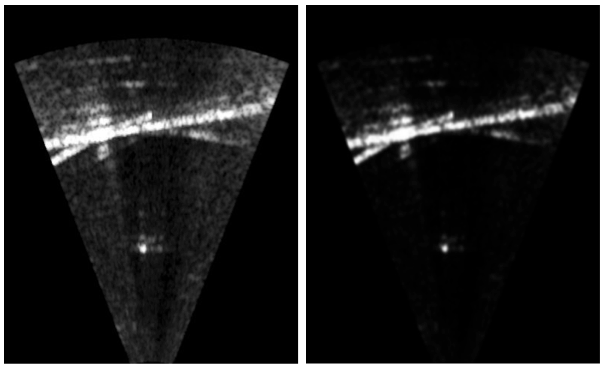
\includegraphics[scale=0.4]{sonarprocessed}
  \captionsetup{justification=centering}
  \caption{Before and after sonar filters}
\end{figure}

Figure 13 shows the image direct from the sensor and after various filters are applied. Several methods used here are referenced from [20]. The first stage was to convolve the image with a 2-D isotropic Gaussian low pass kernel with a $\sigma $ of 5 pixels based on Eq. 11. N and M represent the width and height of the sonar image respectively. This helps remove some of the sparse electrical or acoustic noise in the image. Power law is then applied to the normalized image to enhance brighter regions based on Eq. 12. Finally, image averaging based on Eq. 13 is applied, and helps lower the intensity of sporadic noise that appears in and out of subsequent frames. 
\begingroup\makeatletter\def\f@size{7}\check@mathfonts
\begin{gather}
g\left( x,y \right)\; =\; e^{\frac{-\left( \left( x-c_{x} \right)^{2}+\left( y-c_{y} \right)^{2} \right)}{\left( 2\sigma  \right)^{2}}} \\
c_{x}\; =\; 0.5\cdot N\; c_{y}\; =\; 0.5\cdot M\; \sigma =5\; \nonumber\\
I\left( x,y \right)\; =\; I\left( x,y \right)\otimes g\left( x,y \right) \nonumber\\
I\left( x,y \right)\; =\; \left( \frac{I\left( x,y \right)}{255} \right)^{2}\cdot 255 \\
I\left( x,y \right)\; =\; \frac{\sum_{i}^{2}{I\left( x,y \right)}}{2}
\end{gather}
\endgroup

After these image processing methods, a combination of thresholding, morphology and contour detection is used to extract objects from the image. We can easily extract and track the calibration buoy using these methods as they are distinct from other objects in the image. These  pre-processing techniques will also be later applied before more complex filters such as particle filters are applied. Once the coordinates in the sonar image are extracted, they are passed to the Blueview API to extracr \RSonar and \ThetaSonar.

\subsection{Camera Image processing}

\begin{figure}[h!]
  \centering
  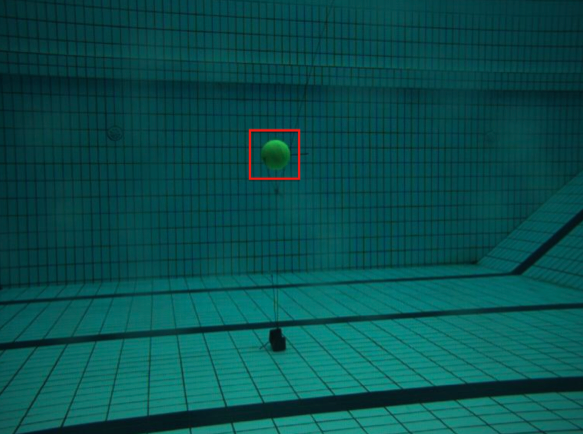
\includegraphics[scale=0.3]{buoycamera}
  \captionsetup{justification=centering}
  \caption{Calibration buoy in camera}
\end{figure}

Camera points are extracted using contrast enhancement, HSV Thresholding to pick out yellow and morphology. This way, we can precisely extract \UCamera and \VCamera automatically. A data collection UI has also been written to extract all this information into a MATLAB friendly format.

\section{Calibration}

\subsection{Calibration process}

A set of data points with (\RSonar, \ThetaSonar, \UCamera, \VCamera), (\RollVehicle, \PitchVehicle, \YawVehicle), (\RollVehicleVelocity, \PitchVehicleVelocity, \YawVehicleVelocity), (\XVehicleVelocity, \YVehicleVelocity, \ZVehicleVelocity) and \YVehicle is collected over a space of 10x2.5x12 metres. A total of 10,000 points was collected over this space and split into 5 datasets consisting of 1 training set and 4 test sets. Camera calibration is conducted to solve for ($f_{x}$, $f_{y}$, $c_{x}, c_{y}$, $K_{1}$,$K_{2}$) on both land and water, and tested to see the that ($f_{x}$, $f_{y}$) differ by 1.33. $L_{z}$, $L_{y}$ and $^{c}T_{s}$ are given initial values which are guessed from the CAD model of the system as seen in Fig 6. The results of this calibration and initial estimation is given in Eq. 14/15. We assume identity for the rotation as it is hard to measure initially.
\begingroup\makeatletter\def\f@size{7}\check@mathfonts
\begin{gather}
F=\left[\begin{array}{cccc}
735.4809 & 0 & 388.9467 & 0\\
0 & 733.6047 & 292.0895 & 0\\
0 & 0 & 1 & 0
\end{array}\right]
 \left[\begin{array}{c}
K_{1}=0.0369\\
K_{2}=-0.3870
\end{array}\right] \\
^{c}T_{s}=\left[\begin{array}{cccc}
1 & 0 & 0 & 0.1\\
0 & 1 & 0 & 0.3\\
0 & 0 & 1 & 0.1\\
0 & 0 & 0 & 1
\end{array}\right]
 \left[\begin{array}{c}
L_{y}=0.2\\
L_{z}=0.4
\end{array}\right]
\end{gather}
\endgroup

The Levenberg Marquardt algorithm [10] for non-linear optimization available in MATLAB is used to minimize Eq. 16 where ($U_{G}$, $V_{G}$) is the ground truth of the yellow buoy, while ($U_{M}$, $V_{M}$) is the camera position calculated from (\RSonar, \ThetaSonar, \YVehicle, \PitchVehicle) based on Eq. 8/10, and initial parameters from Eq. 14/15.
\begingroup\makeatletter\def\f@size{7}\check@mathfonts
\begin{gather}
min(\left(U_{G}-U_{M}\right)^{2}+\left(V_{G}-V_{M}\right)^{2})
\end{gather}
\endgroup

Testing parameters from Eq. 15 against the training set gave results as seen in Fig. 15. The figure on the left shows pixel error from ground truth projection of the yellow buoy vs the combined (\RSonar, \ThetaSonar, \YSonar) projection into the camera. The figure on the right, shows the error in the ground truth 3d coordinates in the vehicle frame, vs that derived from (\RSonar, \ThetaSonar, \YSonar, \UCamera, \VCamera). One can observe significant error in Y direction. After calibration is performed, the newly estimated $L_{z}$, $L_{y}$ and $^{c}T_{s}$ is tested against the training set. Fig. 16 shows significant reduction in error against the ground truth. These results can be better observed in Fig. 17, which shows the 3d error in metres before and after calibration. Fig. 18 shows the error in pixel distance before and after calibration.

Lastly, the newly estimated $L_{z}$, $L_{y}$ and $^{c}T_{s}$ in Eq. 16 is tested against 4 other test sets. Table. 2 shows the mean and variance of the errors before and after calibration of both training and test sets in 3D and Pixel errors. We can observe a 4 time reduction in mean pixel error, and a 6 time reduction in 3D error.

\begin{table}[h]
\small
\resizebox{\columnwidth}{!}{%
\begin{tabular}{|l|l|l|}
\hline
{\bf Data} & {\bf Pixel Error Mean / Var} & {\bf 3D Error Mean / Var}
\\ \hline
\begin{tabular}[c]{@{}l@{}}
Before Calibration \\ Training Set
\end{tabular} &
32.8057 / 43.1141 & 0.1478 / 0.0068
\\ \hline
\begin{tabular}[c]{@{}l@{}}
After Calibration \\ Training Set
\end{tabular} &
8.2440 / 22.7498 & 0.0258 / 0.0007
\\ \hline
\begin{tabular}[c]{@{}l@{}}
After Calibration \\ Test Set 2
\end{tabular} &
8.1873 / 22.3888 & 0.0257 / 0.0007
\\ \hline
\begin{tabular}[c]{@{}l@{}}
After Calibration \\ Test Set 3
\end{tabular} &
8.2730 / 35.4033 & 0.0259 / 0.0008
\\ \hline
\begin{tabular}[c]{@{}l@{}}
After Calibration \\ Test Set 4
\end{tabular} &
8.1897 / 22.2684 & 0.0255 / 0.0007
\\ \hline
\begin{tabular}[c]{@{}l@{}}
After Calibration \\ Test Set 5
\end{tabular} &
8.1486 / 21.5721 & 0.0254 / 0.0007
\\ \hline
\end{tabular}
} \\
\caption{Calibration errors}
\end{table}
\begingroup\makeatletter\def\f@size{7}\check@mathfonts
\begin{gather}
^{c}T_{s}=\left[\begin{array}{cccc}
0.9993 & 0.0311 & 0.0219 & 0.1401\\
-0.0303 & 0.9989 & -0.0363 & 0.2671\\
-0.0230 & 0.0356 & 0.9991 & 0.1407\\
0 & 0 & 0 & 1
\end{array}\right]
 \left[\begin{array}{c}
L_{y}=0.1631\\
L_{z}=0.2473
\end{array}\right]
\end{gather}
\endgroup

\begin{figure*}
  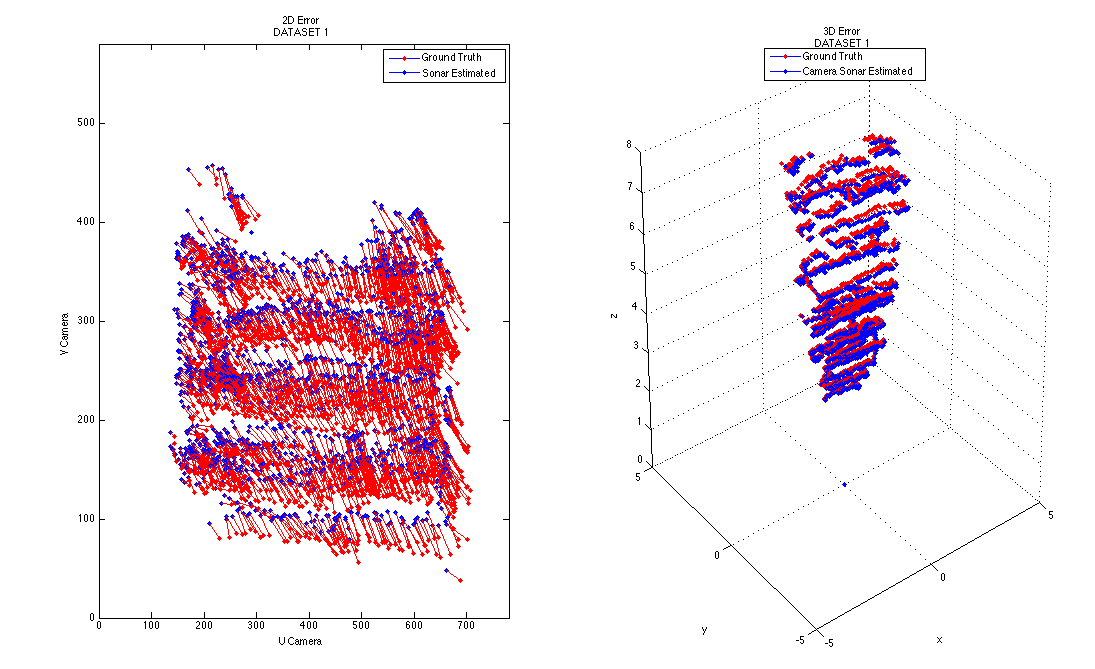
\includegraphics[width=\textwidth,height=8cm]{1}
  \caption{Camera projection error and resolved 3D error before calibration}
\end{figure*}

\begin{figure*}
  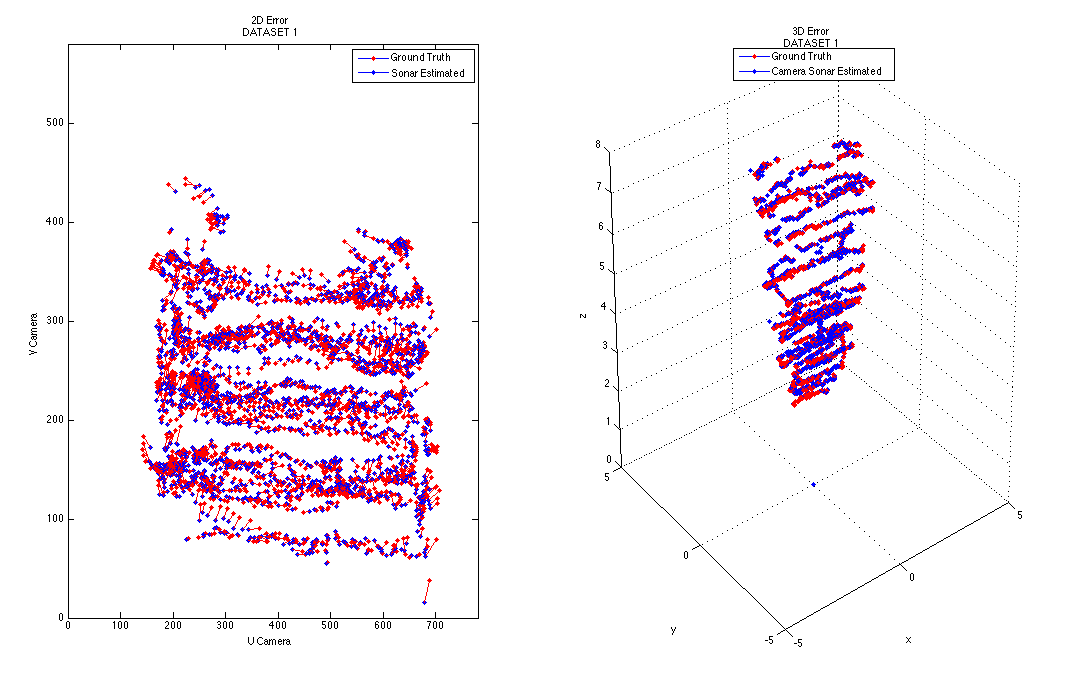
\includegraphics[width=\textwidth,height=8cm]{4}
  \caption{Camera projection error and resolved 3D error after calibration}
\end{figure*}

\begin{figure*}%
\centering
\begin{subfigure}{\columnwidth}
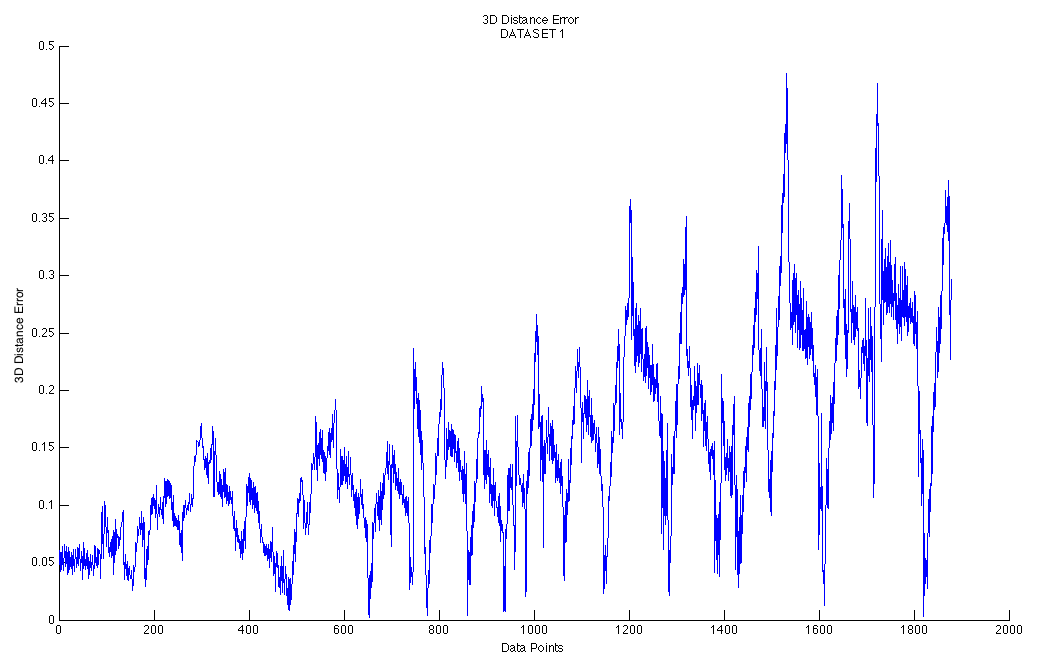
\includegraphics[width=\columnwidth]{3}%
\caption{Before Calibration}%
\label{subfiga}%
\end{subfigure}\hfill%
\begin{subfigure}{\columnwidth}
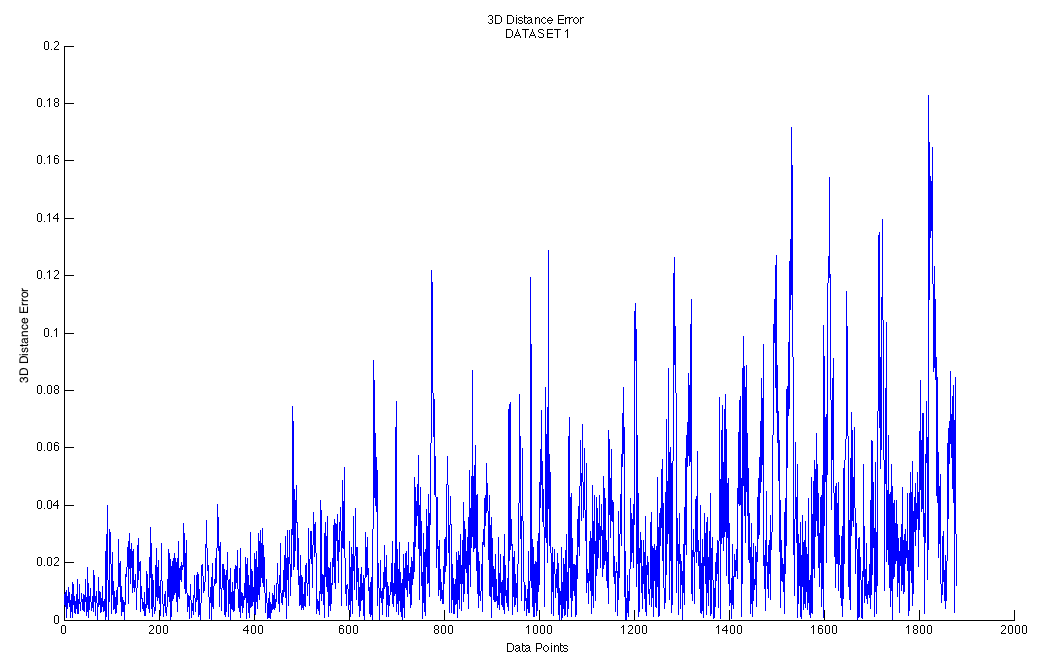
\includegraphics[width=\columnwidth]{6}%
\caption{After Calibration}%
\label{subfiga}%
\end{subfigure}\hfill%
\caption{Distance error between resolved 3d coordinates from sonar and camera data vs ground truth in metres}
\label{figabc}
\end{figure*}

\begin{figure*}
  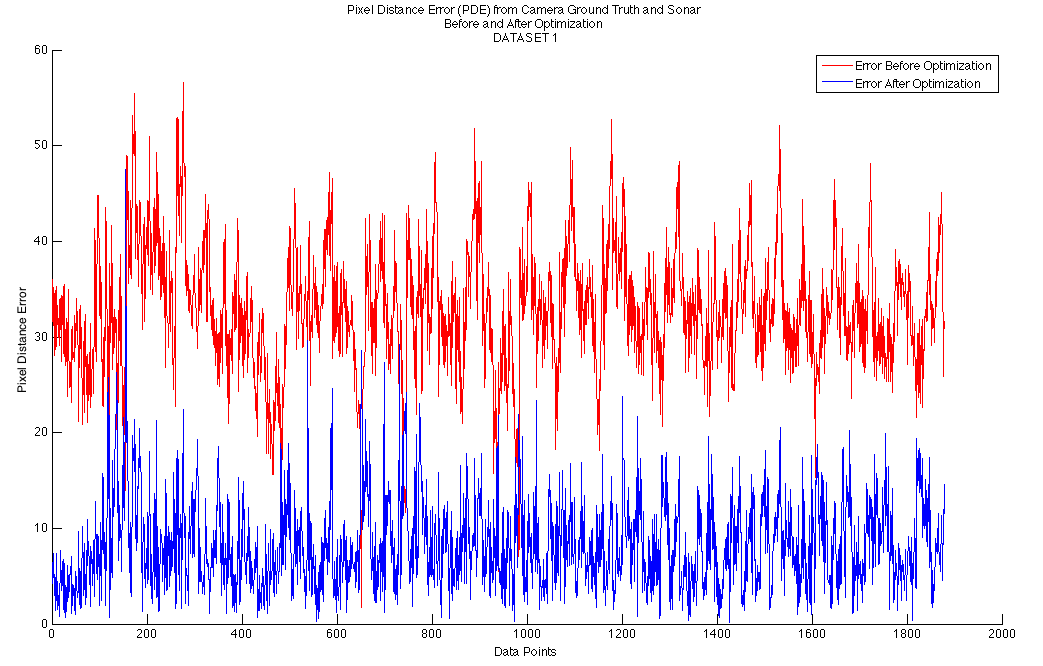
\includegraphics[width=\textwidth,height=10cm]{5}
  \caption{Pixel error between projected pixels before and after calibration}
\end{figure*}

\begin{figure*}%
\centering
\begin{subfigure}{\columnwidth}
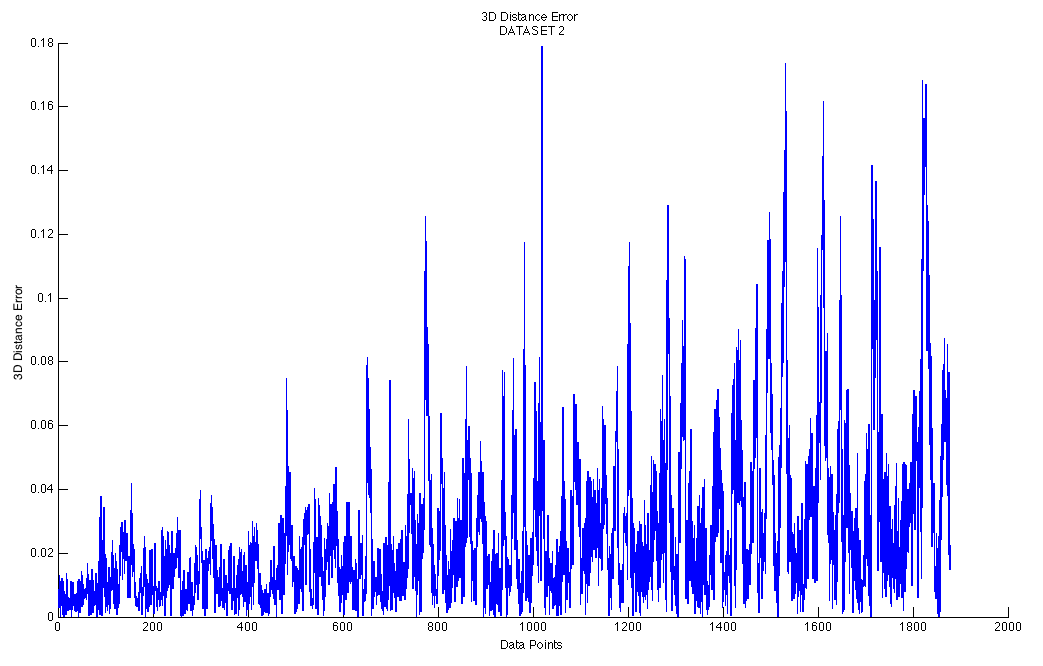
\includegraphics[width=\columnwidth]{T2}%
\caption{3D Error Test Set 2}%
\label{subfiga}%
\end{subfigure}\hfill%
\begin{subfigure}{\columnwidth}
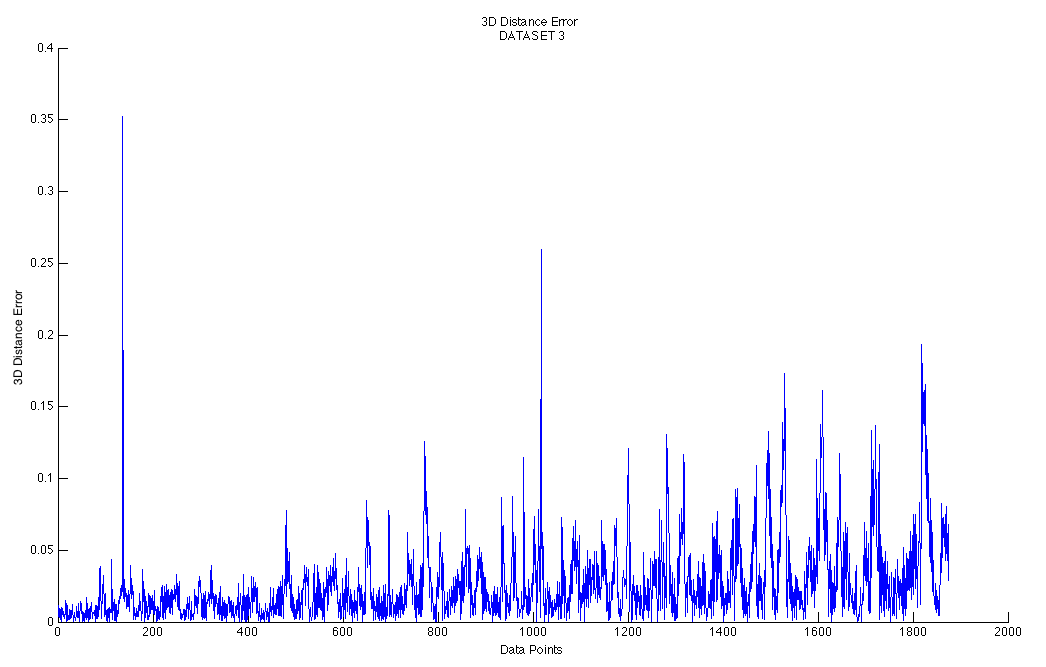
\includegraphics[width=\columnwidth]{T3}%
\caption{3D Error Test Set 3}%
\label{subfiga}%
\end{subfigure}\hfill%
\end{figure*}
\begin{figure*}%
\centering
\begin{subfigure}{\columnwidth}
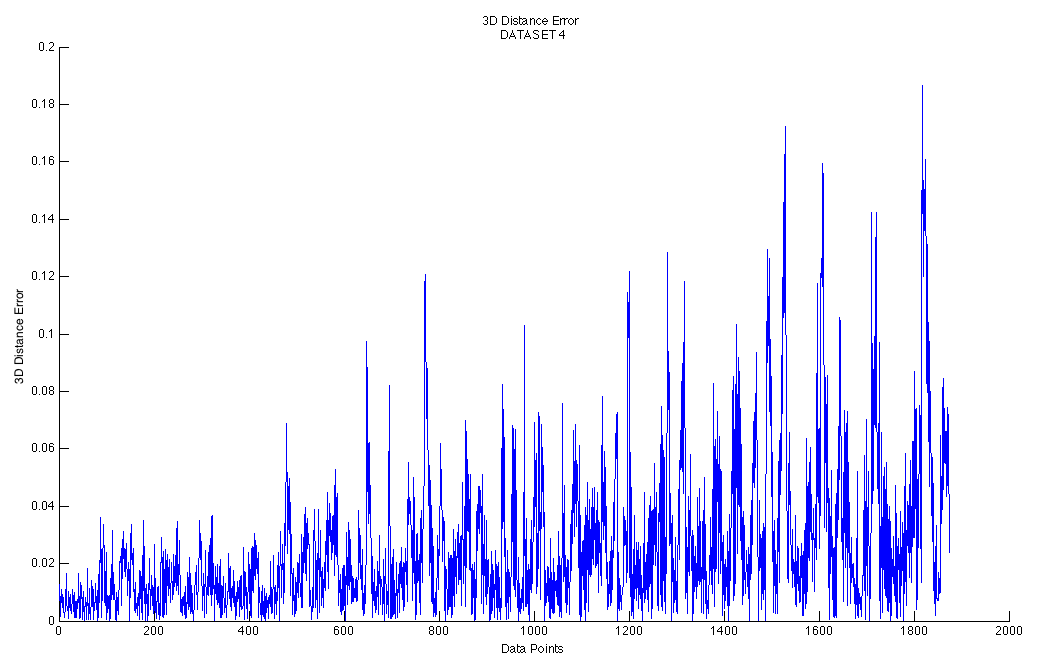
\includegraphics[width=\columnwidth]{T4}%
\caption{3D Error Test Set 4}%
\label{subfiga}%
\end{subfigure}\hfill%
\begin{subfigure}{\columnwidth}
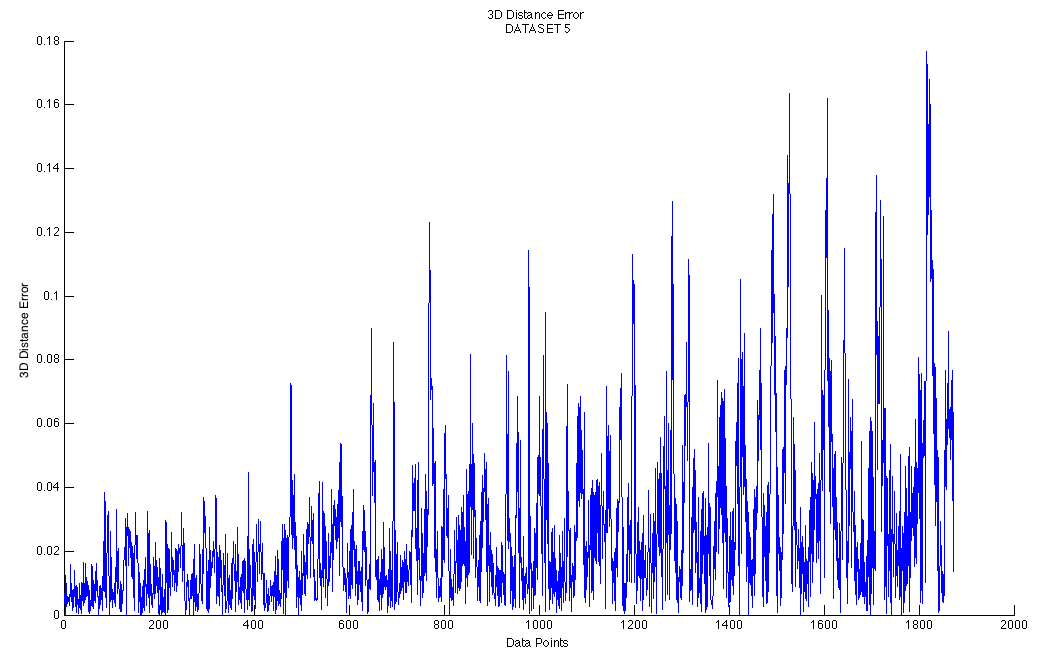
\includegraphics[width=\columnwidth]{T5}%
\caption{3D Error Test Set 5}%
\label{subfiga}%
\end{subfigure}\hfill%
\caption{Testing calibrated parameters derived from training set against 4 test sets}
\label{figabc}
\end{figure*}

\subsection{Real time testing}

Now that we have a mapping between both sensors, we may test this against real time data. In order to solve for (\XVehicle, \YVehicle, \ZVehicle), we need to be able to relate an object on the sonar image with (\RSonar, \ThetaSonar) and an object in the camera (\UCamera, \VCamera). From there, we may solve for \YSonar using Eq. 7. From there, we may compute (\XSonar, \YSonar, \ZSonar) using Eq. 3. Finally, we can use ($L_{z}$, $L_{y}$, \PitchVehicle) to compute (\XVehicle, \YVehicle, \ZVehicle) that may be passed to the control system to actuate the vehicle.

However, we need to relate a blob in the sonar image with a region of interest (ROI) in the camera image in order to compute this. This is done by projecting the corner points and centroid of the sonar blob into the camera as seen in Fig. 21, by extracting (\RSonar, \ThetaSonar) for these 3 points ($A, B, C$), getting the upper and lower \YSonar bounds based on the sonar's min/max elevation, then projecting this as a ambiguity lines into the camera. Then, the ROI from the camera has lines ($A', B', C'$) extracted. Finally, we attempt to iteratively minimize Eq. 18, and selecting the best match. Once the match is known, we can compute the object's coordinates.
\begingroup\makeatletter\def\f@size{7}\check@mathfonts
\begin{gather}
f(A,B) = Distance\ between lines \nonumber\\
\min \left( f\left( A,A' \right)^{2}+f\left( B,B' \right)^{2}+f\left( C,C' \right)^{2} \right)
\end{gather}
\endgroup

\begin{figure}[h!]
  \centering
  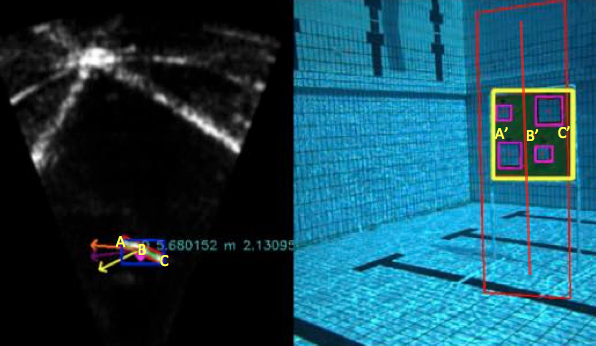
\includegraphics[scale=0.3]{project}
  \captionsetup{justification=centering}
  \caption{Project sonar object into camera}
\end{figure}

This method was used during the AUVSI Robosub 2015 Challenge [21], and proved to be quite effective. However, as noted in the above method, this means of matching both sonar and camera objects requires the ROI in the camera to be extracted accurately. While this method worked in pool conditions, it tended to fail in sea/lake conditions, due to particulate matter in water over large distances, or through temporal irradiance due to sunlight filtering through the water. Also, the vehicle's pitching motion tended to cause the intensity of the sonar object to drop as noted in Eq. 1, causing brief losses in detection due to increased signal to noise ratio. A framework was needed allow for consistent sensing of the object in 3d space.

\section{Tracking Filters}

This is why the need of a statistical tracking filter to track and localize these objects, constrained by the calibrated transformation between both the sonar and camera based on Eq. 7 is proposed and used. Since the objects being tracked are stationary, it is also possible to involve the vehicle's odometry data in order to predict the position of these objects if loss in data occurred in the sonar or camera. 

\subsection{Estimation Theory}

Our problem is to sequentially estimate the state of a dynamic system (in this case our target to be tracked) using noisy measurements from our various sensors. We have a state vector that contains all information required to describe the system (Eg. position and velocity of the object w.r.t the vehicle in 3d space), and we have a measurement vector that contain observations that a related to the state vector through some model (Eg. range and azimuth from the sonar image). A dynamic model is used to describe the system dynamics, such as predicting the next position of an object, and a measurement model is used to relate the measurement and state vectors. Alot of the theory and equations used is extracted from [22].

One way to describe these models is through a Recursive Bayesian Filter, which consists of a prediction and an update stage and assumes the state's uncertainty is distributed through a Gaussian distribution. The prediction step predicts the next pdf using the dynamic model, but uncertainty is added due to system noise (Eg. using odometry data to predict the object's next position has noise), hence stretches the distribution. The update stage then squeezes the distribution using Bayes' theorem. These steps can be described in Eq. 19/20 where $s_{k}$ is the state of the system at time $k$, $f$ is the dynamic model with process noise $w_{k}$ that is used to predict the next state $s_{k+1}$. $h$ is the measurement model with measurement noise $v_{k}$ that is used to correct $s_{k}$.
\begingroup\makeatletter\def\f@size{7}\check@mathfonts
\begin{gather}
s_{k+1}=f(s_{k},w_{k})\quad k\epsilon\mathbb{N} \\
z_{k}=h(s_{k},v_{k})\quad k\epsilon\mathbb{N}
\end{gather}
\endgroup

Given a set of prior observations up to a time $k$, we wish to find the optimal estimate for $s_{k}$. If $p(s_{k}|Z_{k-1})$ is known, the correction step of the pdf can be derived as seen in Eq. 22. If $p(s_{k}|Z_{k})$ is known, the prediction step of the pdf can be derived as seen in Eq. 23. 
\begingroup\makeatletter\def\f@size{7}\check@mathfonts
\begin{gather}
Z_{k}=\{z_{0},...,z_{k}\}=\{Z_{k-1},z_{k}\} \\
p(s_{k}|Z_{k})=\frac{p(Z_{k}|s_{k})p(s_{k})}{p(Z_{k})}=\frac{p(z_{k},Z_{k-1}|s_{k})p(s_{k})}{p(z_{k},Z_{k-1})} \nonumber\\
=\frac{p(z_{k}|s_{k},Z_{k-1})p(Z_{k-1}|s_{k})p(s_{k})}{p(z_{k}|Z_{k-1})p(Z_{k-1})}=\frac{p(z_{k}|s_{k})p(Z_{k-1}|s_{k})p(s_{k})}{p(z_{k}|Z_{k-1})p(Z_{k-1})} \nonumber\\
=\frac{p(z_{k}|s_{k})p(s_{k}|Z_{k-1})}{p(z_{k}|Z_{k-1})} \\
p(s_{k+1},s_{k}|Z_{k})=p(s_{k+1}|s_{k},Z_{k})p(s_{k}|Z_{k})=p(s_{k+1}|s_{k})p(s_{k}|Z_{k}) \nonumber\\
p(s_{k+1}|Z_{k})=\int_{\mathbb{R^{\mathit{n}}}}p(s_{k+1}|s_{k})p(s_{k}|Z_{k})ds_{k}
\end{gather}
\endgroup

The recursive propagation of the pdf can only be done if the system is linear and gaussian, which might not be the case for us. To account for this, one way would be to linearise the system then applying a Kalman Filter (Extended Kalman Filter EKF).

The Kalman Filter assumes that the pdf at every time step is Gaussian, and can be described by a mean and covariance. If we assume the dynamic and measurement models are linear with some gaussian noise added, the filter can be described based on these Eq. 24/25 where $F_{k}$ and $H_{k}$ describe the dynamic and measurement models as linear functions, $w_{k}$, $v_{k}$ and $s_{0}$ are normally distributed based on Eq. 26. 
\begingroup\makeatletter\def\f@size{7}\check@mathfonts
\begin{gather}
s_{k+1}=F_{k}s_{k}+G_{k}w_{k}\quad k\epsilon\mathbb{N} \\
z_{k}=H_{k}s_{k}+v_{k}\quad k\epsilon\mathbb{N} \\
w_{k}\sim N(0,Q_{k}),\quad v_{k}\sim N(0,R_{k}),\quad s_{0}\sim N(\hat{x}_{0},P_{0})
\end{gather}
\endgroup

The Kalman Filter proves that when $Z_{k}$ is given, $s_{k}$ and $s_{k+1}$ are distributed according to Eq. 27/28, and the filter steps is given by Eq. 29. This allows one to recursively compute the mean and covariance of the next state given that the system is linear and gaussian to begin with.
\begingroup\makeatletter\def\f@size{7}\check@mathfonts
\begin{gather}
p(s_{k}|Z_{k})\sim N(\hat{s}_{k|k},P_{k|k}) \\
p(s_{k+1}|Z_{k})\sim N(\hat{s}_{k+1|k},P_{k+1|k}) \\
\hat{s}_{k|k}=\hat{s}_{k|k-1}+P_{k|k-1}H_{k}^{T}S_{k}^{-1}(z_{k}-H_{k}\hat{s}_{k|k-1}) \nonumber\\
P_{k|k}=P_{k|k-1}-P_{k|k-1}H_{k}^{T}S_{k}^{-1}H_{k}P_{k|k-1} \nonumber\\
S_{k}=R_{k}+H_{k}P_{k|k-1}H_{k}^{T} \nonumber\\
\hat{s}_{k+1|k}=F_{k}\hat{s}_{k|k} \nonumber\\
P_{k+1|k}=F_{k}P_{k|k}F_{k}^{T}+W_{k}Q_{k}W_{k}^{T}
\end{gather}
\endgroup

In a nonlinear non-gaussian model, one approach would be to use a particle filter. Here, the pdf is represented as a set of samples with weights. Similar to the first two methods, a dynamic model and a measurement model is used, along with the process and measurement noise based on Eq. 24/25/26. Here however, Monte Carlo (MC) methods are used where the objective is to approximate integrals of the form based on Eq. 30 where $p(s)$ represents a probability function that sums to 1. If we can draw N samples according to $p(s)$, then the integral can be approximated by the sum based on Eq. 31. As $N$ approaches infinity, we can describe the pdf more precisely and we approach an optimal Bayesian estimate. As seen in Fig. 22, particles are able to model multivariate distributions through uneven partitioning, and regions of high/low density.
\begingroup\makeatletter\def\f@size{7}\check@mathfonts
\begin{gather}
I=\int g(s)p(s)ds \\
\hat{I}=\frac{1}{N}\sum_{i=1}^{N}g(s^{i})
\end{gather}
\endgroup

\begin{figure}[h!]
  \centering
  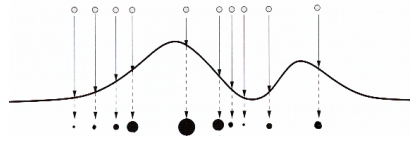
\includegraphics[scale=0.3]{particles}
  \captionsetup{justification=centering}
  \caption{Particle filter estimating pdf}
\end{figure}

\subsection{Particle Filter Algorithm}
\begin{algorithmic}[1]
\STATE \textit{Initialisation} : \\
Generate $N$ particles according to an initial distribution $p_{0}(s_{0})$ set by the user. If not set, assume a uniform distribution over a bounded space.
\STATE \textit{Dynamic Model update} : \\
Time evolution of particles occurs through the dynamic model, with process noise added in.\\
$X_{n|n-1}^{(k)}=f(X_{n-1|n-1}^{(k)},w_{n-1})\quad k\epsilon\mathbb{N}$\\
\STATE \textit{Redistribution} : \\
A certain percentage of particles are then uniformly distributed as suggested by [22] to solve the captured robot problem.
\STATE \textit{Measurement Model update} : \\
Compute weights for each particle given a measurement $Y_{n}$ and normalize \\
$q_{n}=\frac{P(Y_{n}|X_{n|n-1}^{(k)})}{\sum_{k}P(Y_{n}|X_{n|n-1}^{(k)})}\quad k\epsilon\mathbb{N}$
\STATE \textit{Resample} : \\
Generate $N$ new particles by resampling with replacement given a weight $q_{n}$ \\
$X_{n+1|n}^{(k)}=h(X_{n|n}^{(k)}|q_{n})\quad k\epsilon\mathbb{N}$ \\
\STATE Go to step 2 and repeat with new inputs
\end{algorithmic} 

The above steps can be described in Fig. 23, where prediction is done through the dynamic model update in Step. 2/3, calculation and normalization of weights based on the measurement model in Step 4, and resampling in Step 5, in this case done using the computed likelihood histogram based on the normalized weights.

\begin{figure}[h!]
  \centering
  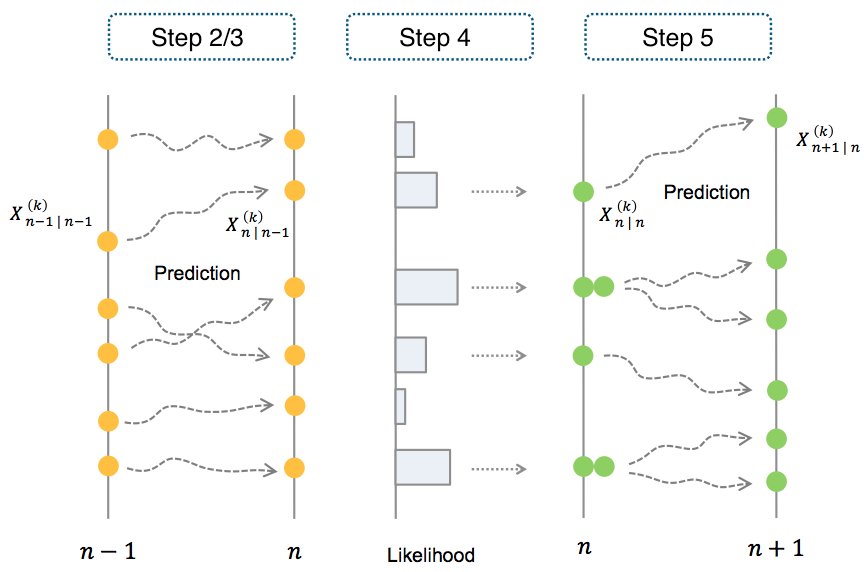
\includegraphics[scale=0.3]{resample}
  \captionsetup{justification=centering}
  \caption{Particle Filter Stages}
\end{figure}

\subsection{Dynamic Model}

The state matrix and dynamic model is given by Eq. 42 which represents the object position and velocity in 3D space in the sonar frame. $N$ number of particles representing possible solutions to where the object is are initially distributed over the workspace as per step 1. Then each particles position is updated based on a simple velocity displacement update matrix with some process noise $w_{k}$ added.
\begingroup\makeatletter\def\f@size{7}\check@mathfonts
\begin{gather}
X_{n|n-1}^{(k)}=\left[\begin{array}{c}
X_{s}\\
Y_{s}\\
Z_{s}\\
\dot{X_{s}}\\
\dot{Y_{s}}\\
\dot{Z_{s}}
\end{array}\right]\quad X_{n|n-1}^{(k)}=\left[\begin{array}{cccccc}
1 & 0 & 0 & T & 0 & 0\\
0 & 1 & 0 & 0 & T & 0\\
0 & 0 & 1 & 0 & 0 & T\\
0 & 0 & 0 & 1 & 0 & 0\\
0 & 0 & 0 & 0 & 1 & 0\\
0 & 0 & 0 & 0 & 0 & 1
\end{array}\right]*X_{n-1|n-1}^{(k)}+w_{n-1}
\end{gather}
\endgroup 

Since the object we are tracking is stationary w.r.t the world frame, we can incorporate the vehicle odometry into the object motion. This is so that if we are unable to measure (\XSonar, \YSonar, \ZSonar) in the measurement step, we can predict the object's next position based on the previous position and current velocity. To do this, we first transform $(X_{s},Y_{s,}Z_{s})_{k}$ at that time instant into the vehicle frame with the known ($L_{y}$, $L_{z}$), and convert it to polar coordinates, based on Eq. 43. We assume the sonar and vehicle frames have an identity rotational component here. 
\begingroup\makeatletter\def\f@size{7}\check@mathfonts
\begin{gather}
\left[\begin{array}{cccc}
1 & 0 & 0 & 0\\
0 & 1 & 0 & L_{y}\\
0 & 0 & 1 & L_{z}\\
0 & 0 & 0 & 1
\end{array}\right]*\left[\begin{array}{c}
X_{s}\\
Y_{s}\\
Z_{s}\\
1
\end{array}\right]_{k}=\left[\begin{array}{c}
X_{v}\\
Y_{v}\\
Z_{v}\\
1
\end{array}\right]_{k}=\left[\begin{array}{c}
R_{v}\cdot\cos\left(\phi_{v}\right)\cdot\sin\left(\theta_{v}\right)\\
R_{s}\cdot\sin\left(\phi_{v}\right)\\
R_{s}\cdot\cos\left(\phi_{v}\right)\cdot\cos\left(\theta_{v}\right)
\end{array}\right]
\end{gather}
\endgroup 

We then differentiate the polar representation of the object in the vehicle frame in Eq. 43 to yield the Jacobian matrix in Eq. 44. 
\begingroup\makeatletter\def\f@size{7}\check@mathfonts
\begin{gather}
\left[\begin{array}{c}
\dot{X_{v}}\\
\dot{Y_{v}}\\
\dot{Z_{v}}
\end{array}\right]=\frac{d}{dt}\left[\begin{array}{c}
R_{v}\cdot\cos\left(\phi_{v}\right)\cdot\sin\left(\theta_{v}\right)\\
R_{v}\cdot\sin\left(\phi_{v}\right)\\
R_{v}\cdot\cos\left(\phi_{v}\right)\cdot\cos\left(\theta_{v}\right)
\end{array}\right]= \nonumber\\
\left[\begin{array}{c}
\left(\dot{R_{v}}\cdot\cos\left(\phi_{v}\right)\cdot\sin\left(\theta_{v}\right)\right)-\left(R_{v}\cdot\dot{\phi_{v}}\cdot\sin\left(\phi_{v}\right)\cdot\sin\left(\theta_{v}\right)\right)+\left(R_{v}\cdot\dot{\theta_{v}}\cdot\cos\left(\phi_{v}\right)\cdot\cos\left(\theta_{v}\right)\right)\\
\left(\dot{R_{s}}\cdot\sin\left(\phi_{v}\right)\right)+\left(R_{v}\cdot\dot{\phi_{v}}\cdot\cos\left(\phi_{v}\right)\right)\\
\left(\dot{R_{v}}\cdot\cos\left(\phi_{v}\right)\cdot\cos\left(\theta_{v}\right)\right)-\left(R_{v}\cdot\dot{\phi_{v}}\cdot\sin\left(\phi_{v}\right)\cdot\cos\left(\theta_{v}\right)\right)-\left(R_{v}\cdot\dot{\theta_{v}}\cdot\cos\left(\phi_{v}\right)\cdot\sin\left(\theta_{v}\right)\right)
\end{array}\right]
\end{gather}
\endgroup 

Next, some components in the Jacobian matrix are replaced with their equivalent readings of other sensors as seen in Eq. 45. The $\dot{R_{v}}$ components are equal to the negative vehicular translational velocity components, and the $\dot{\theta_{v}}$ and $\dot{\phi_{v}}$ are equal to the negative angular velocities of pitch and yaw. This yields Eq. 46, which shows the replaced values.
\begingroup\makeatletter\def\f@size{7}\check@mathfonts
\begin{gather}
\left[\begin{array}{c}
\left(\dot{R_{v}}\cdot\cos\left(\phi_{v}\right)\cdot\sin\left(\theta_{v}\right)\right)\\
\left(\dot{R_{v}}\cdot\sin\left(\phi_{v}\right)\right)\\
\left(\dot{R_{v}}\cdot\cos\left(\phi_{v}\right)\cdot\cos\left(\theta_{v}\right)\right)
\end{array}\right]=\left[\begin{array}{c}
\dot{-X_{v}}\\
\dot{-Y_{v}}\\
\dot{-Z_{v}}
\end{array}\right]\quad\left[\begin{array}{c}
\dot{\theta_{v}}\\
\dot{\phi_{v}}
\end{array}\right]=\left[\begin{array}{c}
\dot{-\gamma_{v}}\\
\dot{-\beta_{v}}
\end{array}\right] \\
\left[\begin{array}{c}
\dot{X_{v}}\\
\dot{Y_{v}}\\
\dot{Z_{v}}
\end{array}\right]=\left[\begin{array}{c}
\left(\dot{-X_{v}}\right)-\left(R_{v}\cdot\dot{-\beta_{v}}\cdot\sin\left(\phi_{v}\right)\cdot\sin\left(\theta_{v}\right)\right)+\left(R_{v}\cdot\dot{-\gamma_{v}}\cdot\cos\left(\phi_{v}\right)\cdot\cos\left(\theta_{v}\right)\right)\\
\left(\dot{-Y_{v}}\right)+\left(R_{v}\cdot\dot{-\beta_{v}}\cdot\cos\left(\phi_{v}\right)\right)\\
\left(\dot{-Z_{v}}\right)-\left(R_{v}\cdot\dot{-\beta_{v}}\cdot\sin\left(\phi_{v}\right)\cdot\cos\left(\theta_{v}\right)\right)-\left(R_{v}\cdot\dot{-\gamma_{v}}\cdot\cos\left(\phi_{v}\right)\cdot\sin\left(\theta_{v}\right)\right)
\end{array}\right]
\end{gather}
\endgroup

We then perform the the update/prediction step based on the velocity model in Eq. 42, then transform the newly estimated $(X_{v},Y_{v,}Z_{v})_{k+1}$ back into the sonar frame $(X_{s},Y_{s,}Z_{s})_{k+1}$ as seen in Eq. 47.
\begingroup\makeatletter\def\f@size{7}\check@mathfonts
\begin{gather}
\left[\begin{array}{cccc}
1 & 0 & 0 & 0\\
0 & 1 & 0 & -L_{y}\\
0 & 0 & 1 & -L_{z}\\
0 & 0 & 0 & 1
\end{array}\right]*\left[\begin{array}{c}
X_{v}\\
Y_{v}\\
Z_{v}\\
1
\end{array}\right]_{k+1}=\left[\begin{array}{c}
X_{s}\\
Y_{s}\\
Z_{s}\\
1
\end{array}\right]_{k+1}
\end{gather}
\endgroup 

\subsection{Measurement Model}

Now that we have predicted the new position of the object (\XSonar, \YSonar, \ZSonar) using the dynamic model above, we wish to correct this with measurements from the sonar and camera. In order to do this, we project this data into their respective image pixels since their calibration data is known. Fig. 24 shows the particles in the sonar frame projected into the sonar image by converting (\XSonar, \YSonar, \ZSonar) into (\RSonar, \ThetaSonar, \PhiSonar). \RSonar and \ThetaSonar may then be matched into the sonar image pixel coordinates provided by the Blueview API. (\XSonar, \YSonar, \ZSonar) are then transformed into the camera frame and projected into the camera based on the calibration data derived as seen in Eq. 48/49. From here, we can extract ($U_{s}, V_{s}$) and ($U_{c}, V_{c}$) pixel coordinates in both sensors from the particle state.
\begingroup\makeatletter\def\f@size{7}\check@mathfonts
\begin{gather}
\left[\begin{array}{c}
\sqrt{X_{s}^{2}+Y_{s}^{2}+Z_{s}^{2}}\\
arctan(\frac{X_{s}}{Y_{s}})\\
arctan(\frac{Y_{s}}{\sqrt{X_{s}^{2}+Y_{s}^{2}+Z_{s}^{2}}})
\end{array}\right]=\left[\begin{array}{c}
R_{s}\\
\Theta_{s}\\
\Phi_{s}
\end{array}\right]=>\left[\begin{array}{c}
U_{s}\\
V_{s}
\end{array}\right] \\
\left[\begin{array}{cccc}
735.4809 & 0 & 388.9467 & 0\\
0 & 733.6047 & 292.0895 & 0\\
0 & 0 & 1 & 0
\end{array}\right]*\left[\begin{array}{cccc}
0.9993 & 0.0311 & 0.0219 & 0.1401\\
-0.0303 & 0.9989 & -0.0363 & 0.2671\\
-0.0230 & 0.0356 & 0.9991 & 0.1407\\
0 & 0 & 0 & 1
\end{array}\right]* \nonumber\\
\left[\begin{array}{c}
X_{s}\\
Y_{s}\\
Z_{s}
\end{array}\right]=>\left[\begin{array}{c}
U_{c}\\
V_{c}
\end{array}\right]
\end{gather}
\endgroup 

Computing the weight of the particles from the sonar image is done by taking ($U_{s}, V_{s}$) and testing that pixel against several features, such as brightness/intensity of that spot and major/minor axis of the shape of the object that pixel is in. This shape information such as the major/minor axis length is extracted by performing contour analysis, morphology and oriented bounding box fitting via Principle Component Analysis (PCA) [24].

This is done by calculating the log likelihood of that particle/state where we assume the above features that are measured at a particular state follow a gaussian distribution given a user specified major/minor axis length. This is specified by Eq. 40/41. Here, $d$ represents the difference between a user specified measurement and actual measurement.
\begingroup\makeatletter\def\f@size{7}\check@mathfonts
\begin{gather}
P(Y_{n}|X_{n|n-1}^{(k)})=\frac{1}{\sqrt{2\pi\sigma^{2}}}\cdot exp(-\frac{d^{2}}{2\sigma^{2}}) \\
log(P(Y_{n}|X_{n|n-1}^{(k)}))=-log(\sigma\sqrt{2\pi})-\frac{0.5}{\sigma^{2}}\cdot d^{2}
\end{gather}
\endgroup 

The final sonar weight of a particle is given by Eq. 42 where Fig. 24 describes the features used.
\begingroup\makeatletter\def\f@size{7}\check@mathfonts
\begin{gather}
q_{n}^{sonar}=-log(\sigma_{Intensity}\sqrt{2\pi})-\frac{0.5}{\sigma_{Intensity}^{2}}\cdot((U_{s},V_{s})_{Intensity}-255)^{2}+ \nonumber\\
-log(\sigma_{MajorAxis}\sqrt{2\pi})-\frac{0.5}{\sigma_{MajorAxis}^{2}}\cdot((U_{s},V_{s})_{MajorAxis}-User_{MajorAxis})^{2}+ \nonumber\\
-log(\sigma_{MinorAxis}\sqrt{2\pi})-\frac{0.5}{\sigma_{MinorAxis}^{2}}\cdot((U_{s},V_{s})_{MinorAxis}-User_{MinorAxis})^{2}
\end{gather}
\endgroup 

\begin{figure}[h!]
  \centering
  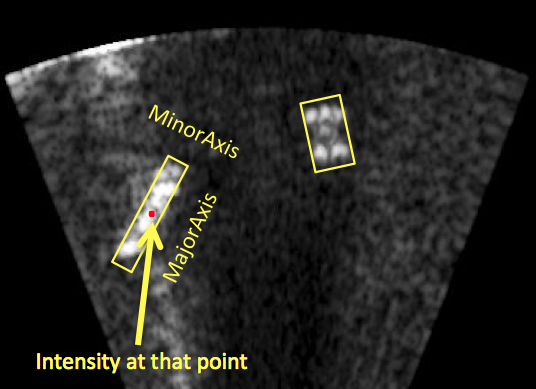
\includegraphics[scale=0.3]{majorminor}
  \captionsetup{justification=centering}
  \caption{Sonar Features used}
\end{figure}

Computing the weight of the particles from the camera image is done by taking ($U_{c}, V_{c}$) and testing that pixel against several features, such as hue and shape ratio. The final camera weight of a particle is given by Eq. 43.
\begingroup\makeatletter\def\f@size{7}\check@mathfonts
\begin{gather}
q_{n}^{camera}=-log(\sigma_{Hue}\sqrt{2\pi})-\frac{0.5}{\sigma_{Hue}^{2}}\cdot((U_{c},V_{c})_{Hue}-User_{Hue})^{2}+ \nonumber\\
-log(\sigma_{Ratio}\sqrt{2\pi})-\frac{0.5}{\sigma_{Ratio}^{2}}\cdot((U_{c},V_{c})_{Ratio}-User_{Ratio})^{2}
\end{gather}
\endgroup 

There is also the possibility of computing the Pixel Velocity using the Lucas-Kanade feature tracking method, and giving higher weights to the projected particles that match this velocity, but using the above features were found to be sufficient. We finally add these weights up, perhaps giving more weightage to either sensor in the fusion process if the user requires it, and normalize it as per step 4. Lastly, resampling with replacement is then applied as per step 5 and the process is repeated.
\begingroup\makeatletter\def\f@size{7}\check@mathfonts
\begin{gather}
P(Y_{n}|X_{n|n-1}^{(k)})=q_{n}^{sonar}+q_{n}^{camera} \\
q_{n}=\frac{P(Y_{n}|X_{n|n-1}^{(k)})}{\sum_{k}P(Y_{n}|X_{n|n-1}^{(k)})}\quad k\epsilon\mathbb{N}
\end{gather}
\endgroup 

\subsection{Particle Filter Results}

Fig. 25 to Fig. 27 shows the particle filter algorithm in action tested in pool conditions. One can observe that initially, there is ambiguity in \PhiSonar as the object wasn't visible in the camera. As the vehicle moves closer, the ambiguity is corrected. Finally, as the object moves out of the sonar image, we can see the ambiguity in \RSonar. Also, in instances wgere there is loss of information from either sensor, we are still able to predict the next position of the object using the vehicle odometry data.

Fig. 28 to Fig. 30 show the particle filter algorithm in action tested in murky water conditions with poor visibility in the camera imagery, and a low SNR in the sonar imagery due to the object being almost out of the sonar frustum as seen in Fig. 29. Despite this, the particles still converge on the correct solution over time. It is also impervious to noise from surrounding wall as seen in Fig. 30. 

We can see the mapping vs particle filter tracking results on Fig. 32 for both cases. The mapping algorithm loses alot of data points as it requires testing the ROI extracted from the camera against the projected ROI of the sonar object. This method still worked well in the first case in pool conditions, but failed miserably in murky water conditions. Using the particle filter method however, we can observe much better results that fill in alot of the gaps of the first method.

\begin{figure*}
  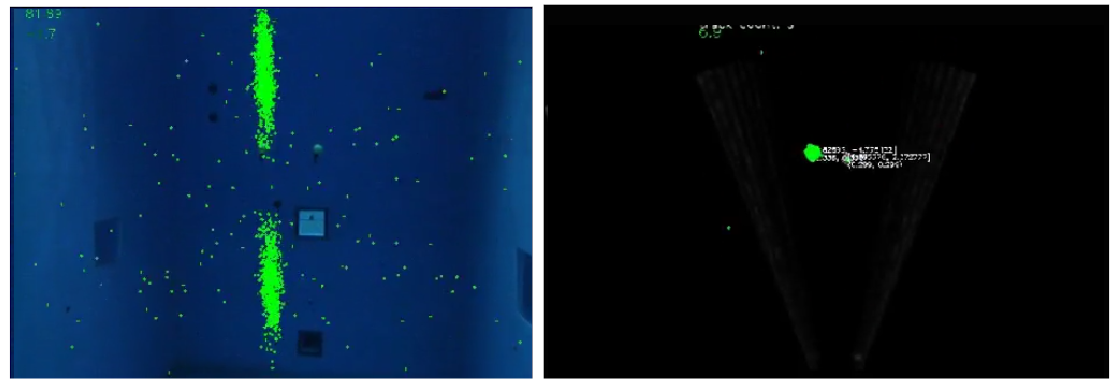
\includegraphics[width=\textwidth,height=8cm]{pfraw3}
  \caption{Object not visible in camera, hence ambiguity in elevation}
  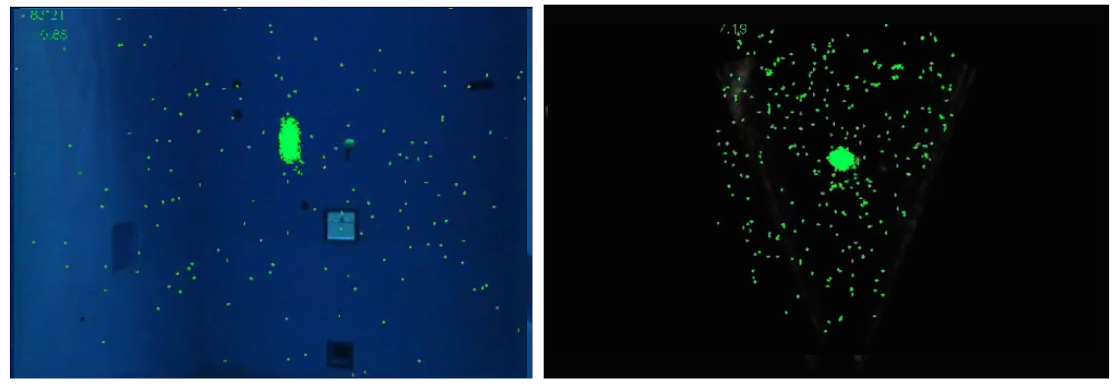
\includegraphics[width=\textwidth,height=8cm]{pfraw4}
  \captionsetup{font=small,skip=-10pt,justification=centering}
  \caption{Elevation ambiguity corrected via camera. Also loss of sonar information at that instant, but position still maintained through camera and odometry fusion but with increased covariance}
  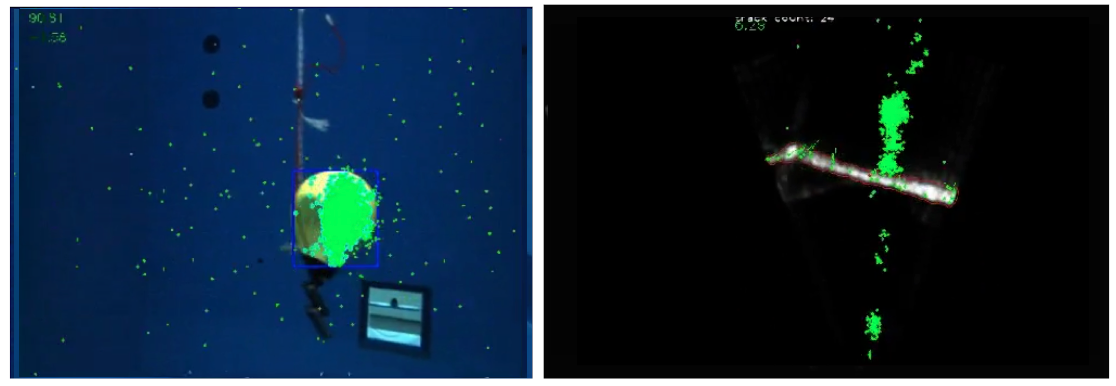
\includegraphics[width=\textwidth,height=8cm]{pfraw5}
  \captionsetup{font=small,skip=-10pt,justification=centering}
  \caption{Object not visible in sonar, hence ambiguity in range}
\end{figure*}

\begin{figure*}
  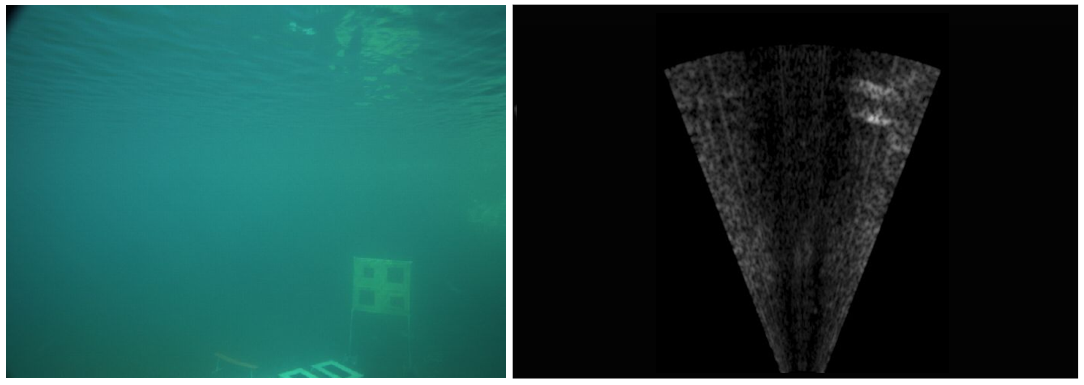
\includegraphics[width=\textwidth,height=8cm]{pfsem1}
  \caption{Objective is to localize the task board located nearly 15m away in murky water and is barely visible in either sensor}
  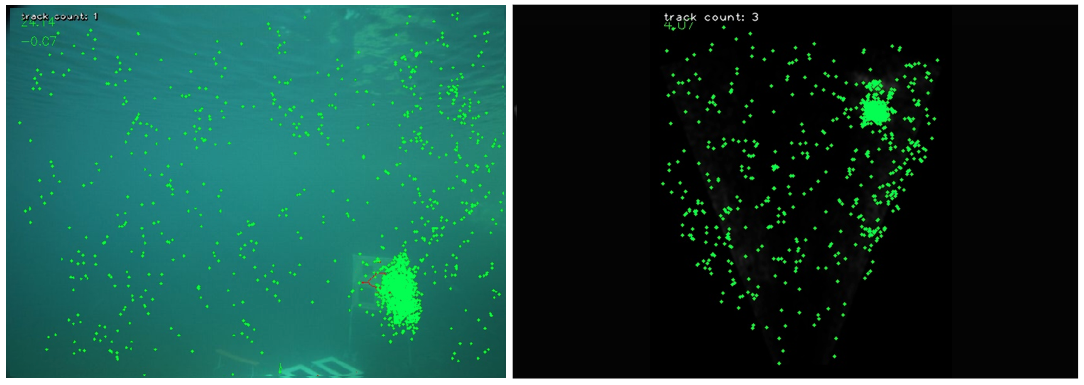
\includegraphics[width=\textwidth,height=8cm]{pfsem2}
  \caption{Particle Filter still localizes the object in 3D space}
  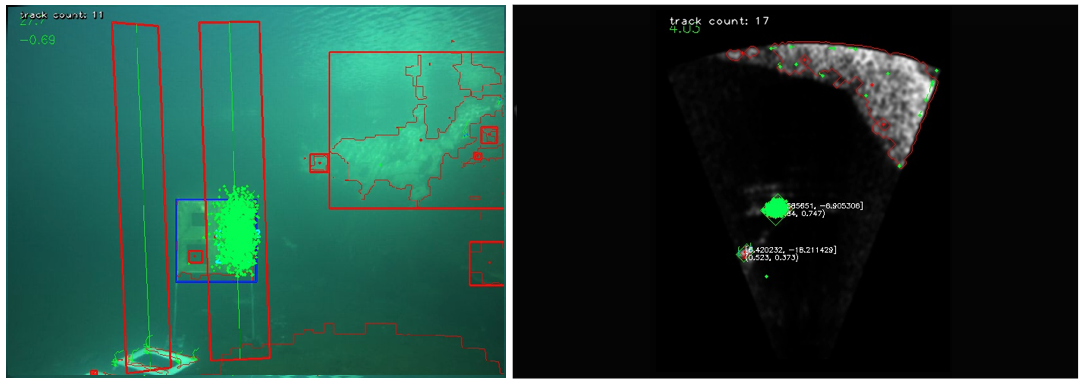
\includegraphics[width=\textwidth,height=8cm]{pfsem3}
  \captionsetup{font=small,skip=-10pt,justification=centering}
  \caption{Particle Filter localizes the object despite noisy data in both sensors when close to a wall}
\end{figure*}

\begin{figure*}%
\centering
\begin{subfigure}{\columnwidth}
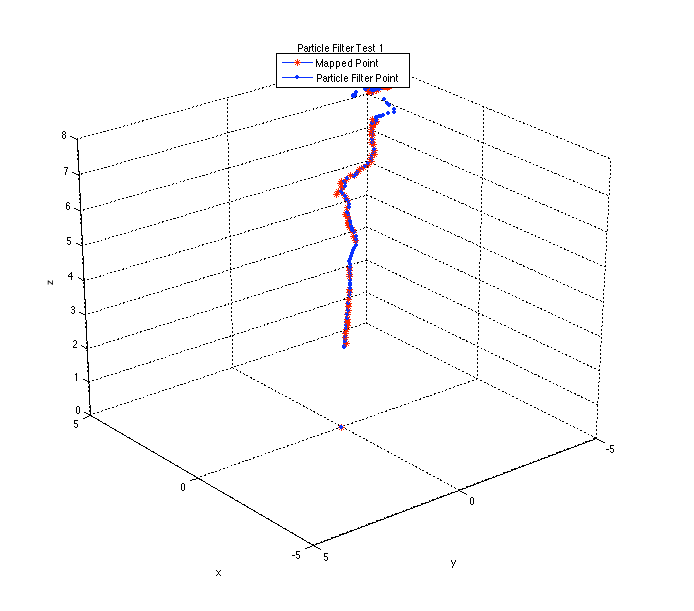
\includegraphics[width=\columnwidth]{pfo2}%
\caption{Pool conditions}%
\end{subfigure}\hfill%
\begin{subfigure}{\columnwidth}
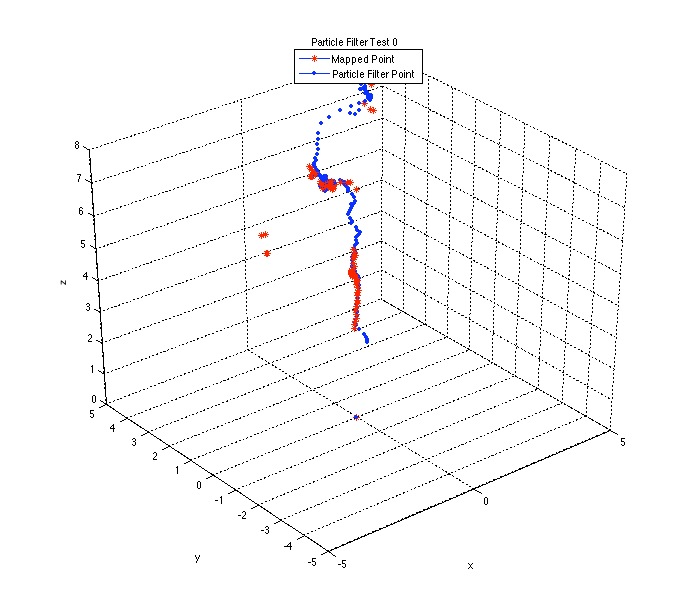
\includegraphics[width=\columnwidth]{pfo1}%
\caption{Murky water conditions}%
\label{subfiga}%
\end{subfigure}\hfill%
\end{figure*}
\begin{figure*}%
\centering
\caption{Comparison of object coordinates derived through the mapping method vs particle filter}
\label{figabc}
\end{figure*}
 
\section{Conclusion}

This paper proposed a novel algorithm using the rising edge in combination with the phase information of an acoustic ping to estimate its source location. The algorithm was validated through implementation as a real time system on the BumbleBee Autonomous Underwater Vehicle. 
The resulting algorithm was found to meet the specifications of the system stated in the beginning of the project, in particular the requirements for. The estimation of distance, although outperforming what could be done with just a Rising Edge based algorithm, can still be improved upon further. 
Future work can be done to further evaluate the use of other methods to further enhance the estimation of distance. A larger number of sensors would allow for more robust estimation with less fluctuation due to the increased redundancy in information, possibly allowing for reliable distance estimation at larger distances. A different sensor array configuration could This paper proposed a novel algorithm using the rising edge in combination with the phase information of an acoustic ping to estimate its source location. The algorithm was validated through implementation as a real time system on the BumbleBee Autonomous Underwater Vehicle. 
The resulting algorithm was found to meet the specifications of the system stated in the beginning of the project, in particular the requirements for. The estimation of distance, although outperforming what could be done with just a Rising Edge based algorithm, can still be improved upon further. 
Future work can be done to further evaluate the use of other methods to further enhance the estimation of distance. A larger number of sensors would allow for more robust estimation with less fluctuation due to the increased redundancy in information, possibly allowing for reliable distance estimation at larger distances. A different sensor array configuration could also possibly be implemented to improve the distance estimate. 


% EQUATIONS ARE WRONG NUMBER. DO THE EXP THING%

% References
\begin{thebibliography}{1}

\bibitem{IEEEhowto:kopka}
Y. Swirski and Y. Y. Schechner, “3Deflicker from motion,” 2013 IEEE Int. Conf. Comput. Photogr. ICCP 2013, 2013.

\bibitem{IEEEhowto:kopka}
N. Carlevaris-Bianco, A. Mohan, and R. M. Eustice, “Initial results in underwater single image dehazing,” MTS/IEEE Seattle, Ocean. 2010, 2010.

\bibitem{IEEEhowto:kopka}
http://www.blueview.com/products/2d-imaging-sonar/p450-series/

\bibitem{IEEEhowto:kopka}
S. Williams, and Ian Mahon. "Simultaneous localisation and mapping on the great barrier reef." In Robotics and Automation, 2004. Proceedings. ICRA'04. 2004 IEEE International Conference on, vol. 2, pp. 1771- 1776. IEEE, 2004. 

\bibitem{IEEEhowto:kopka}
G. H. Xu, L. Y. Wu, K. Yu, C. Yang, and L. Yang, “Multi-target Detection of Underwater Vehicle Based on Multi-sensor Data Fusion,” vol. 4, pp. 467–471, 2012.

\bibitem{IEEEhowto:kopka}
A. Spears, A. M. Howard, M. West, and T. Collins, “Acoustic Sonar and Video Sensor Fusion for Landmark Detection in an Under-Ice Environment.”

\bibitem{IEEEhowto:kopka}
D. W. Krout, G. Okopal, and E. Hanusa, “Video data and sonar data : real world data fusion example,” Inf. Fusion (FUSION), 2011 Proc. 14th Int. Conf., pp. 1 – 5, 2011. 

\bibitem{IEEEhowto:kopka}
S. Negahdaripour, H. Sekkati, and H. Pirsiavash. "Opti-acoustic stereo imaging: On system calibration and 3-D target reconstruction." Image Processing, IEEE Transactions on 18, no. 6 (2009): 1203-1214.

\bibitem{IEEEhowto:kopka}
S. Negahdaripour, “A new method for calibration of an opti-acoustic stereo imaging system,” MTS/IEEE Seattle, Ocean. 2010, pp. 1–7, 2010.

\bibitem{IEEEhowto:kopka}
D. Marquardt, “An algorithm for least-squares estimation of nonlinear parameters,” J. SIAM, vol. 11, no. 2, 1963.

\bibitem{IEEEhowto:kopka}
http://www.bbauv.com/wp-content/uploads/2014/06/paper-1.pdf

\bibitem{IEEEhowto:kopka}
E. Coiras and J. Groen, “Simulation and 3d reconstruction of sidelooking sonar images,” Adv. sonar Technol. IN-TECH, no. February, pp. 1–15, 2009.

\bibitem{IEEEhowto:kopka}
V. Creuze, B. Jouvencel, and P. Baccou, “3D-bottom tracking based on acoustic diffraction for autonomous underwater vehicles,” ICAR ’05. Proceedings., 12th Int. Conf. Adv. Robot. 2005., pp. 3–8, 2005.

\bibitem{IEEEhowto:kopka}
V. Creuze, B. Jouvencel, and P. Baccou, “3D-bottom tracking based on acoustic diffraction for autonomous underwater vehicles,” ICAR ’05. Proceedings., 12th Int. Conf. Adv. Robot. 2005., pp. 3–8, 2005.

\bibitem{IEEEhowto:kopka}
P. F. Sturm and S. J. Maybank, “On plane-based camera calibration: A general algorithm, singularities, applications,” Proceedings. 1999 IEEE Comput. Soc. Conf. Comput. Vis. Pattern Recognit. (Cat. No PR00149), vol. 1, no. c, 1999.

\bibitem{IEEEhowto:kopka}
D. M. Deveau and A. P. Lyons, "Fluid-filled passive sonar calibration spheres: design, modeling, and measurement," IEEE J. Oceanic Eng., vol. 34, pp. 93-100, 2009.

\bibitem{IEEEhowto:kopka}
Stefan van der Walt, S. Chris Colbert and Gael Varoquaux. The NumPy Array: A Structure for Efficient Numerical Computation, Computing in Science and Engineering ,13, 22-30 (2011), DOI:10.1109/MCSE.2011.37

\bibitem{IEEEhowto:kopka}
M. Quigley, K. Conley, B. Gerkey, J. FAust, T. Foote, J. Leibs, E. Berger, R. Wheeler, and A. Mg, “ROS: an open-source Robot Operating System,” Icra, vol. 3, no. Figure 1, p. 5, 2009.

\bibitem{IEEEhowto:kopka}
G. Bradski. The OpenCV Library. Dr. Dobb’s Journal of Software Tools, 2000.

\bibitem{IEEEhowto:kopka}
K. Kim, D. Seo, and H. Kim, “Radar target identification using one-dimensional scattering centres,” IEE Proceedings-Radar, Sonar Navig., vol. 152, no. 4, pp. 285–296, 2001.

\bibitem{IEEEhowto:kopka}
www.auvsifoundation.org/foundation/competitions/robosub/

\bibitem{IEEEhowto:kopka}
J. Torstensson and M. Trieb, “Particle Filtering for Track Before Detect Applications,” 2005.

\bibitem{IEEEhowto:kopka}
D. Fox, W. Burgard, F. Dellaert, and S. Thrun, “Monte Carlo Localization: Efficient Position Estimation for Mobile Robots Dieter Fox, Wolfram Burgard,” 16th Natl. Conf. Artif. Intell., no. Handschin 1970, pp. 343–349, 1999.

\bibitem{IEEEhowto:kopka}
L.-Y. Weng, M. Li, Z. Gong, and S. Ma, “Underwater object detection and localization based on multi-beam sonar image processing,” 2012 IEEE Int. Conf. Robot. Biomimetics, pp. 514–519, 2012.

\end{thebibliography}

\end{document}
